\cotefile{136}
\scanpage{95}
\begin{center}- \mspage{169} -\end{center}
\margin{IX}

finies ; donc $X\longmapsto\widehat X$ transforme groupes en groupes. Notons que $\widehat X$ ne dépend en fait que de la restriction de $X$ à un voisinage ouvert arbitraire $U$ de $S$.

\uline{Lemme} 13.2.1. \uline{Les données sont celles de} 13.1, \uline{et on suppose que les conditions suivantes sont vérifiées} : a) $A=A^0$, b) $R$ \uline{est constant au voisinage de} $s$, \uline{et} c) $R_s$ \uline{engendre l'espace vectoriel complexe} $E_s$. \uline{Soit} $A'$ \uline{un deuxième groupe analytique lisse sur} $S$, \uline{et considérons l'application}
\[
u\longmapsto\widehat u:\operatorname{Hom}_{S\text{-}\mathrm{gr}}(A,A')\longrightarrow\operatorname{Hom}_{\widehat S\text{-}\mathrm{gr}}(\widehat A,\widehat {A'})\quad,
\]
\uline{où les notations sont celles de} 13.2, \uline{et l'application analogue obtenue en se restreignant au-dessus d'un voisinage ouvert} $U$ \uline{variable de} $s$, \uline{et passant à la limite inductive} :
\[
(13.2.1.1)\qquad u\longmapsto\widehat u:\operatorname{Hom}_{(S,s)\text{-}\mathrm{gr}}(A,A')\longrightarrow\operatorname{Hom}_{\widehat S\text{-}\mathrm{gr}}(\widehat A,\widehat {A'})\quad,
\]
(\uline{où} $(S,s)$ \uline{désigne le} germe \uline{d'espace analytique de} $S$ \uline{en} $s$). \uline{Alors l'application précédente est} bijective.

Considérons en effet la suite exacte
\diagram{\begin{tikzcd}
0\arrow[r]&R'\arrow[r]&E'\arrow[r]&A'{}^0\arrow[r]&0
\end{tikzcd}}
analogue à (13.1.3) définie par $A'$. Compte tenu du fait que les homomorphismes $A\longrightarrow A'$ se factorisent nécessairement par $A'{}^0$, et de même après les changements de base $U\longrightarrow S$ et $S_n\longrightarrow S$, on peut supposer $A'=A'{}^0$. Compte tenu du dictionnaire 13.1.4, il faut prouver que la donnée d'un

\margin{\unsure{487}\ \illegible{2}}
\margin{487}
\margin{94}

\scanpage{96}
\diagram{\begin{tikzcd}[row sep=small,column sep=small]
0&0&0&\\
0&0&A^{2\,2}&\text{---}\\
0&A^{1\,1}&A^{2\,1}\arrow[u]&\text{---}\\
k&A^{1\,0}\arrow[u]&A^{2\,0}\arrow[u]&\cdots
\end{tikzcd}}

Soit $A^{**}\in\operatorname{Ob}\mathrm{DR}_{\unsure{\mathrm{sp}}}(X,k)$

$T\in\Gamma_X(A^{1,0})$ définit
$\begin{array}{rcl}k&\longrightarrow&A^{1,0}=\Phi,\\\lambda&\longmapsto&\lambda T\end{array}$,
\unsure{on a suite} exacte
\diagram{\begin{tikzcd}
0\arrow[r,dash]&k\arrow[r]&\Phi\arrow[r]\arrow[d,equal]&\Psi\arrow[r]\arrow[d,dash]&0\\
&&A^{1\,0}&A^{\unsure{2\,0}}
\end{tikzcd}}
Comme $\Psi$ est $k$-plat, $\Phi$ \unsure{aussi} et on sait que
\[
\mathrm{DR}(\Phi,T)=\underbrace{\Gamma^*(\Phi)}_{\text{deg}\atop\text{compl.}}\otimes_k\underbrace{\bigwedge^*\Psi}_{\text{deg ext.}}
\]
\unsure{muni} des \deleted{\unsure{str.}} \inserted{\unsure{structures}} habituelles est une $k$-alg. de De Rham \unsure{spéciale} et on a un $k$-hom. canonique de telles
\[
\mathrm{DR}(\Phi,T)\longrightarrow A^{**}
\]
\deleted{donc la cat. de}

Un hom $A^{**}\unsure{-|\longrightarrow}A'{}^{**}$ définit diagramme commutatif
\diagram{\begin{tikzcd}
\mathrm{DR}(\Phi,T)\arrow[r]\arrow[d]&A^{**}\arrow[d]\\
\mathrm{DR}(\Phi',T')\arrow[r]&A'{}^{**}
\end{tikzcd}}
Cela \unsure{implique} aisément que la cat. dérivée $\mathrm{DR}_{\unsure{\mathrm{sp}}}(X,k)_0$ est \unsure{équivalente} canoniquement à la \deleted{\unsure{sous-}}catégorie \inserted{dérivée} \unsure{déduite} des algèbres de la forme $\mathrm{DR}(\Phi,T)$, qui est aussi celle des suites exactes
\diagram{\begin{tikzcd}
0\arrow[r]&k\arrow[r]&\Phi\arrow[r]&\Psi\arrow[r]&0
\end{tikzcd}}
avec $\Psi$ plat sur $k$.

\margin{95}

\scanpage{97}
\begin{center}- \mspage{156} -\end{center}
\margin{IX}
\[
(12.4.2)\qquad d(x_i)=C'_i-C''_i\quad,
\]
$C'_i$ et $C''_i$ étant les deux composantes irréductibles de $\widetilde C$ qui correspondent aux branches passant par le point double $x_i$. L'opérateur $d$ dépend du choix de l'ordre $(C'_i,C''_i)$ qu'on se donne entre ces deux branches, et l'isomorphisme (12.4.1) dépend évidemment de ce système de choix. Cependant, si pour $i\in I$ on désigne par
\[
(12.4.3)\qquad\varphi_{x_i}:M\longrightarrow\mathbb Z
\]
le composé $M\longrightarrow\mathbb Z^I\xrightarrow{\mathrm{pr}_i}\mathbb Z$, où le premier homomorphisme provient de (12.4.1), on constate aussitôt (en revenant à l'expression (12.3.4)) que $\varphi_{x_i}$ est bien déterminé au signe près ; de façon plus précise, il dépend seulement de l'ordre pris entre les deux branches $C'_i,C''_i$ passant par $i$, et change de signe quand on change cet ordre. Il s'ensuit notamment que la forme bilinéaire
\[
(12.4.4)\qquad\varphi_{x_i}\otimes\varphi_{x_i}\in\check M\otimes_{\mathbb Z}\check M\simeq\operatorname{Hom}(M\otimes M,\mathbb Z)
\]
est déterminée canoniquement en termes du point singulier $x_i$, sans ambiguïté de signe. On peut donc poser
\figure{\begin{tikzpicture}\draw[->] (0.7,0)--(0,0);\end{tikzpicture}}
\[
(12.4.5)\qquad u=\sum_i\varphi_{x_i}\otimes\varphi_{x_i}:M\otimes_{\mathbb Z}M\longrightarrow\mathbb Z\quad,
\]
et on trouve ainsi un accouplement bien déterminé i.e. indépendant de tout choix de signes. Il est clair qu'il est \uline{défini positif}, car c'est la restriction à $M\hookrightarrow\mathbb Z^I$ de la forme quadratique standart $\sum X_i^2$ sur $\mathbb Z^I$.

\margin{474}
\margin{474}
\margin{96}

\scanpage{98}
On sait que cette dernière est équivalente à la cat. ponctuelle. Donc $\mathrm{DR}_{\unsure{\mathrm{sp}}}(X,k)_0$ est équivalente à la cat. ponctuelle.

Si maintenant on travaille \unsure{des|dans} $\mathrm{DR}_{\unsure{\mathrm{spufl}}}$ \deleted{(\unsure{noté} $\mathrm{DR}_{\unsure{\mathrm{spfl}}}$)} i.e. avec des $A^{**}$ \inserted{u.} flasques, ($A^{ij}$ \inserted{u.} flasque si $\unsure{i<j}$) donc $\Phi$ est \inserted{u.} flasque.
\deleted{(\unsure{pour}\ \unsure{flasque})}.

Supposons que ceci implique que les $\Gamma_k^i\Phi$ $(i>0)$ sont uni. flasques, alors $\mathrm{DR}(\Phi,T)$ est aussi flasques, \deleted{et} et même univ. flasque, et on voit comme dessus que la cat. dérivée est équiv. à celle construite avec \deleted{la cat. des} $\mathrm{DR}(\Phi,T)$, avec $\Phi$ univ. flasque et $\Phi/k.T$ plat, i.e. avec les suites exactes
\diagram{\begin{tikzcd}
0\arrow[r]&k\arrow[r]&\Phi\arrow[r]&\Psi\arrow[r]&0
\end{tikzcd}}
avec $\Phi$ univ. flasque et $\Psi$ $k$-plat ; or cette cat. dérivée est encore la catégorie ponctuelle. On trouve donc

\uline{Prop} La cat. $\mathrm{DR}_{\unsure{\mathrm{sp}}}(X,k)_0$ est équivalente à la cat. ponctuelle. Il en est de même de la cat. $\mathrm{DR}_{\unsure{\mathrm{spufl}}}(X,k)_0$, si on suppose que pour tout \inserted{$k$-Module} $\Phi$ plat et univ. flasque, les $\Gamma^i\Phi$ $(i>0)$ sont aussi univ. flasques.

\margin{97}

\scanpage{99}
\begin{center}- \mspage{167} -\end{center}
\margin{IX}
$A$ \uline{lisse} sur $S$, et on désigne par
\[
(13.1.1)\qquad\underline E=\underline{\operatorname{Lie}}(A/S)
\]
le module localement libre sur $S$, image inverse par la section nulle du faisceau tangent relatif de $A$ sur $S$. Nous admettrons ici la définition de l'homomorphisme exponentiel
\[
(13.1.2)\qquad\exp:E\longrightarrow A\quad,
\]
où $E$ est le fibré vectoriel analytique sur $S$ dont le Module des sections holomorphes est $\underline E$. Cet homomorphisme se définit, au voisinage d'un point $s\in S$, d'abord au voisinage de la section nulle de $E$ par les méthodes bien connues en théorie des groupes formels en car. nulle, puis se prolonge de façon évidente par multiplicativité à $E$ tout entier. C'est un homomorphisme de groupes analytiques relatifs sur $S$, qui est \uline{étale} et a comme image le sous-espace ouvert $A^0$ de $A$ réunion des composantes neutres des fibres de $A$ sur $S$. Si $R$ est le sous-espace analytique noyau de $\exp$, on a donc une suite exacte de groupes analytiques relatifs :
\[
(13.1.3)\qquad
\diagram{\begin{tikzcd}0\arrow[r]&R\arrow[r]&E\arrow[r]&A^0\arrow[r]&0\end{tikzcd}}\quad,
\]
où le morphisme $E\longrightarrow A^0$ est surjectif et étale, donc $R$ est un groupe analytique relatif \uline{étale} sur $S$. C'est un sous-espace analytique de $E$, qui est fermé dans $E$ si et seulement si $A^0$ est séparé sur $S$, i.e. la section nulle de $A^0$ est fermée dans $A^0$.

\margin{485}
\margin{485}
\margin{98}

\scanpage{100}
Cette dernière condition est satisfaite pour le topos \inserted{$(S_s=)$} $\widehat\Delta$, car pour celui-ci
\[
\underbrace{\text{flasque}+\text{plat}\inserted{\uline{\unsure{non, projectif|lire projectif}}}}_{\Downarrow}\Longrightarrow\text{homotope à }0,
\]
donc \unsure{univ. flasque} et les $\Gamma^i(\Phi)$ univ. flasques $(i>0)$.
\margin{faux tel quel, à arranger}

Soit $P$ le topos ponctuel, et
\[
i_n:P\longrightarrow\widehat\Delta\ (S_s)
\]
le morphisme de topos associé au foncteur fibre
\[
i_n^*(K)=K_n=K(\Delta_n).
\]
Soit $k$ un anneau (constant)

\uline{Lemme} $\forall$ $k$-module $M$, on a un isom. can.
\[
i_{0*}(M)\simeq\Phi_*\otimes_{\mathbb Z}M\simeq\Phi_{*k}\otimes_k M
\]
où $\Phi_*\in\operatorname{Ob}(\widehat\Delta_{\mathrm{ab}}\simeq\operatorname{Hom}(\Delta^\circ,\mathrm{Ab.}))$ est défini par $\Phi_*(I)=\mathbb Z^I$, \unsure{donc|d'où} $\Phi_{*k}(I)\simeq k^I$.

En effet, on a par construction de l'image directe
\[
\begin{array}{ccc}
i_{0*}(M)(I)&\simeq M(i_0^*(I))&\simeq M^I\\
\Vert&\Vert&\\
\operatorname{Hom}(I,i_{0*}(M))&\operatorname{Hom}(\underbrace{i_0^*(I)}_{\operatorname{Hom}(\Delta_0,I)\simeq I},M)&
\end{array}
\]
\margin{OK.}
\deleted{\unsure{Soit le}}
\uline{Corollaire} Pour tout $k_*$-Module $A_*$, on a
\[
\operatorname{Hom}_{k_*}(A_*,\Phi_{*k}\otimes_k M)\simeq\operatorname{Hom}_k(A_0,M)
\]
en particulier on a un hom can. (\unsure{pour} $M=\unsure{C_0|A_0}$)
\[
\deleted{\unsure{Hom}}\quad A_*\longrightarrow\Phi_*\otimes_{\mathbb Z}A_0\simeq\Phi_{*k}\otimes_k A_0\ (=i_{0*}i_0^*A_*)
\]
Appliquons ceci au cas d'un monomorphisme
\[
k_*\xrightarrow{u} A_*=A_*^{1,0}
\]
provenant d'une $A_*^{**}\in\operatorname{Ob}\mathrm{DR}_{\unsure{\mathrm{sp}}}(S_s,k_*)$

\margin{99}

\scanpage{101}
\begin{center}- \mspage{171} -\end{center}
\margin{IX}
engendre $R$ au voisinage de $s$, d'où il résulte que $F(R)\subset R'$ au voisinage de $s$, ce qui achève la démonstration.

\uline{Corollaire} 13.2.2. \uline{Si} $A$ \uline{satisfait les conditions} a), b), c) \uline{de} 13.2.2, \uline{il est déterminé à isomorphisme unique près au voisinage de} $s$ \uline{par la connaissance du} $\widehat S$-\uline{groupe} $\widehat A$.

13.3. \uline{L'extension de Raynaud analytique}. Nous sommes maintenant en mesure de paraphraser, en Géométrie Analytique, la construction de l'extension de Raynaud donnée dans 7. Supposons donné $A$ comme dans 13.1, avec $A=A_0$, et considérons $R_0=R_s$, qui est un $\mathbb Z$-module libre de type fini. Quitte à restreindre $S$ à un voisinage ouvert assez petit de $s$, interprétant $R_0$ comme le groupe des germes de sections de $R$ au voisinage de $s$, on trouve $\overline{\text{un}}$ homomorphisme
\[
(13.3.1)\qquad R_{0S}\longrightarrow R\subset E
\]
où $R_{0S}$ désigne le groupe analytique constant sur $S$ de valeur $R_0$. Choisissant le voisinage de $s$ assez petit pour que toute section de $\underline{\mathrm O}_S$ dont le germe en $s$ est nul soit nul, on voit que l'homomorphisme précédent est injectif. Son image est donc un \uline{sous}-groupe analytique constant de $R$, qui est évidemment le plus grand sous-groupe constant de $R$, et qui s'appelle la partie \uline{fixe} de $R$, et est notée $R^f$ :
\[
(13.3.2)\qquad R_{0S}\simeq R^f\unsure{\subset|\hookrightarrow}R,\ \text{induit un isomorphisme }R^f_s\simeq R_s.
\]
On pourra alors considérer le groupe quotient
\[
(13.3.3)\qquad A^{\natural}=E/R^f
\]
\margin{\unsure{489}}
\margin{489}
\margin{100}

\scanpage{102}
\deleted{Considérons l'hom induit en degré $0$}
\[\deleted{k_0=k\longrightarrow A_0}\]
On trouve donc un hom
\diagram{\begin{tikzcd}
A_*\arrow[r]&\Phi_*\otimes_{\mathbb Z}A_0\\
k_*\arrow[u,hook]\arrow[r,hook]&\Phi_{*k}\ (=\Phi_*\otimes_{\mathbb Z}k)\arrow[u,hook,"{\Phi_*\otimes_{\mathbb Z}u_0}"']
\end{tikzcd}}
\margin{donnant lieu à un diag. comm.}
Ainsi on trouve un diagramme canonique d'hom dans $\mathrm{DR}_{\unsure{\mathrm{sp}}}(S_s,k_*)$
\diagram{\begin{tikzcd}
\mathrm{DR}(A_*^{1\,0},T)\arrow[r]\arrow[d]&A_*^{**}\\
\mathrm{DR}(A_0^{1\,0}\otimes_{\mathbb Z}\Phi_*,T)&\mathrm{DR}(\Phi_{*k},\overset{\nearrow}{T})\arrow[l]
\end{tikzcd}}
reliant une ``algèbre de DR. spéciale, en $3$ crans, à l'algèbre de DR standart $\mathrm{DR}(\Phi_{*k},T)$ (qui semble \unsure{la plus|le plus} économique de toutes). Si $A_*^{**}$ est \inserted{(univ)} flasque, alors il en est de même de $\mathrm{DR}(A_*^{1\,0},T)$, et le diagramme ci-dessus se trouve dans $\mathrm{DR}_{\unsure{\mathrm{spufl}}}$.

On va introduire maintenant les catégories $\mathrm{DR}_{\mathrm{sp}}'(X,k)$, $\mathrm{DR}_{\mathrm{spufl}}'(X,k)$ ayant les mêmes objets que les catégories sans $'$, mais ayant plus de morphismes : les hom. de $k$-algèbres \deleted{\unsure{graduées}} \inserted{différentielles} \deleted{\illegible{2}} à p.d. \unsure{respectant} $T$

\margin{101}

\scanpage{103}
\begin{center}- \mspage{166} -\end{center}
\margin{IX}
qui n'est autre que 12.5 dans le cas de $\underline X^\lambda$ sur $\underline S^\lambda$. Or $\underline S$ est un trait de \uline{caractéristique nulle}. Cela achève donc la réduction annoncée.

\uline{Remarques} 12.9. On notera que cette réduction nous réduit en même temps au cas où $X_0$ n'a qu'un seul point singulier, qui est celui qui était considéré classiquement dans la formule de Picard-Lefschetz. Notons d'ailleurs que dans ce cas, $X_0$ a une ou deux composantes irréductibles, ces cas correspondants respectivement à $\operatorname{rang}M=1$ et $\operatorname{rang}M=0$ (ce dernier cas étant celui où la jacobienne de la fibre générique a bonne réduction).

12.10. La démonstration donnée dans 12.8 nous fournit un résultat plus général que 12.5, valable sans supposer que $X$ soit régulier, en introduisant les entiers $d_\lambda\geq1$ de (12.8.12) : on trouve alors que les accouplements de monodromie se déduisent tous de l'accouplement
\[
(12.10.1)\qquad u=\sum_{\lambda\in L}d_\lambda\varphi_{x_\lambda}\otimes\varphi_{x_\lambda}:M\otimes M\longrightarrow\mathbb Z\quad.
\]

13. \uline{Liens avec la théorie transcendante} : \uline{cas analytique complexe}.

Pour les notions générales relatives aux espaces analytiques, nous renvoyons à [2].

13.1. \uline{Rappels sur les groupes analytiques sur} $S$. Soit $S$ un espace analytique, $A$ un espace analytique au-dessus de $S$, muni d'une structure de groupe commutatif au-dessus de $S$ (i.e. $A$ est un groupe commutatif de la catégorie des espaces analytiques au-dessus de $S$). On suppose

\margin{484}
\margin{484}
\margin{102}

\scanpage{104}
\[
u:\underbrace{\widehat A^{**}}_{\Vert\ \prod A^{ij}}\unsure{-|\longrightarrow}\underbrace{\widehat {A'}{}^{**}}_{\Vert\ \prod A'{}^{ij}}
\]
hom d'Anneaux différentiels appliquant $A^{**+}$ dans $A'{}^{**+}$ et compatible aux p.d., et tels que $u(T)=T$ \unsure{NB} a priori
\[
u:\underbrace{k\{T\}}_{\Vert\ H^*(A^{**})}\longrightarrow\underbrace{k\{T\}}_{\Vert\ H^*(A'{}^{**})}
\]
hom compatible aux p.d.). \deleted{À vrai dire, il \unsure{se peut}\ \unsure{déduire de ce qui précède}}

On désigne par
\[
\mathrm{DR}_{\mathrm{sp}}'(X,k)_0,\quad\mathrm{DR}_{\mathrm{spufl}}'(X,k)_0
\]
les cat. dérivées associées (i.e. les groupoïdes engendrés). On a un \deleted{\unsure{des}} diagramme comm. de foncteurs
\diagram{\begin{tikzcd}[row sep=large,column sep=large]
\mathrm{DR}_{\mathrm{sp}}(X,k)\arrow[r,"{\text{surj. sur obj}}"]\arrow[d,"{\deleted{\unsure{iso.}}\ \text{surjectif sur obj}}"]&\mathrm{DR}_{\mathrm{sp}}(X,k)_0\simeq\text{ponctuelle}\arrow[d]\\
\mathrm{DR}_{\mathrm{sp}}'(X,k)\arrow[r,"{\text{surj. sur objet}}"']&\mathrm{DR}_{\mathrm{sp}}'(X,k)_0\\
\mathrm{DR}_{\mathrm{spufl}}(X,k)\arrow[r,"{\text{surj. sur obj}}"]\arrow[uu,bend left=25,"{\deleted{\unsure{\downarrow}}}"']\arrow[d,"{\text{surjectif sur obj}}"]&\mathrm{DR}_{\mathrm{spufl}}(X,k)_0\simeq\text{ponct.}\arrow[uu,bend left=25,"{\unsure{\uparrow|\downarrow}}"]\arrow[d,"{\text{(si ufl. stable par les }\Gamma^i,\ i>0\text{)}}"]\\
\mathrm{DR}_{\mathrm{spufl}}'(X,k)\arrow[r,"{\text{surj. sur ob}}"]\arrow[uu,bend left=25,"{\deleted{\unsure{\downarrow}}}"']&\mathrm{DR}_{\mathrm{spufl}}'(X,k)_0\simeq\arrow[uu,bend left=25,"{\deleted{\unsure{\downarrow}}}"]
\end{tikzcd}}
qui montre que les deux catégories \inserted{\unsure{dér.}} $\mathrm{DR}_{\mathrm{sp}}'(X,k)_0$ et $\mathrm{DR}_{\mathrm{spufl}}'(X,k)_0$ sont des groupoïdes \inserted{\unsure{ens.}} \unsure{ponctuels|pointés} (munis d'une foule d'objets avec syst. transitif d'iso. entre). Donc ils sont \unsure{can.}

\margin{103}

\scanpage{105}
\begin{center}- \mspage{170} -\end{center}
\margin{IX}
germe d'homomorphisme de fibrés vectoriels $E\longrightarrow E'$, appliquant $R$ dans $R'$, revient à la donnée d'un système cohérent d'homomorphismes $E_n\longrightarrow E'_n$ appliquant $R_n$ dans $R'_n$. Or si $\underline{\mathrm O}_s$ désigne l'anneau local de $S$ en $s$, la donnée d'un système cohérent d'homomorphismes $E_n\longrightarrow E'_n$ revient à la donnée d'un homomorphisme de $\widehat{\underline{\mathrm O}}_s$-modules
\[
\widehat F:\widehat{\underline E}_s\longrightarrow\widehat{\underline E'}_s
\]
(où $\underline E_s$ et $E'_s$ sont les $\underline{\mathrm O}_s$-modules libres fibres en $s$ des $\underline{\mathrm O}_S$-Modules $\underline E$, $\underline E'$ correspondant à $E,E'$), tandis qu'un germe d'homomorphisme de fibrés vectoriels $E\longrightarrow E'$ revient à la donnée d'un homomorphisme de $\underline{\mathrm O}_s$-modules
\[
F:\underline E_s\longrightarrow\underline E'_s\quad.
\]
Cela montre déjà que l'application (13.2.1.1) est injective, et pour la surjectivité, il suffit de prouver que si on a un homomorphisme $\widehat F$ comme dessus, tel que pour tout $n$ l'homomorphisme induit $F_n:E_n\longrightarrow E'_n$ applique $R_n$ dans $R'_n$, alors $\widehat F$ provient d'un $F$ i.e. applique $\underline E_s$ dans $\underline E'_s$, et le germe correspondant d'homomorphismes $E\longrightarrow E'$ applique $R$ dans $R'$. Or, comme par hypothèse c), $R_s=R_0$ engendre $E_s$, il s'ensuit par Nakayama que le groupe $R_0$ (identifié au groupe des sections de $\widehat R$ sur $\widehat S$, ou,au choix,au groupe des germes de sections de $R$ sur $S$) engendre $\widehat E_s$ ; donc, pour prouver que $\widehat F(\underline E_s)\subset\underline E'_s$,il suffit de prouver que $\widehat F(R_0)\subset\underline E'_s$. Or on a $\widehat F(R_0)\subset R'_0$, où $R'_0$ est lui-même interprété comme le groupe des germes de sections de $R'\subset E'$ au voisinage de $s$, d'où l'inclusion annoncée, et par suite l'existence de $F$. De plus on voit que $F(R_0)\subset R'_0$, où $R_0$ et $R'_0$ sont considérés comme des groupes de germes de sections de $E$ resp. $E'$. En vertu de b), $R_0$

\margin{\diagram{\begin{tikzcd}
\mathrm{DR}(A^{1,0},T)\arrow[r]\arrow[d]&A^{**}\\
\mathrm{DR}(\unsure{\Phi_*}\otimes_{\mathbb Z}A_0,T)&\\
{}\arrow[u]&
\end{tikzcd}}}
\margin{488}
\margin{488}
\margin{104}

\scanpage{106}
\unsure{équivalents} à des groupoïdes connexes définis par deux groupes, que nous nous proposons de déterminer [dans le cas $X=S_s$].
\diagram{\begin{tikzcd}
\widehat A_*^{**}\arrow[r,"u"]&\widehat {A'}_*^{**}\\
\widehat{\mathrm{DR}}(\underbrace{A_*^{1\,0}}_{\Vert\ (A_*)},T)\arrow[u]\arrow[ur,dashed,"v"']&\\
\widehat{\Gamma^*}(A_*)\widehat\otimes_k\widehat{\bigwedge^*}(\underbrace{B_*}_{\Vert\ A_*/k_*})\arrow[u,equal]&
\end{tikzcd}}
\[
\begin{array}{rcl}A_*&\xrightarrow{v}&A'{}^{**+}\\T&\longmapsto&T\end{array}
\]
\[
v(p,q):A_*\longrightarrow A'{}^{pq}\qquad(p,q\geq0,\ p+q>0)
\]
\[
v(1,0)(T)=T
\]
\[
v(p,q)(T)=0\quad\text{si }(p,q)\neq(1,0)
\]
\[
\overline v(p,q):B\longrightarrow A'{}^{pq}\qquad\text{(si }\unsure{(p+q)|(p,q)}\neq(1,0)\text{)}
\]
\diagram{\begin{tikzcd}
k\arrow[r,hook]\arrow[d,equal]&A\arrow[d,"{v(1,0)}"]\\
k\arrow[r,hook]&A'{}^{1,0}
\end{tikzcd}}
\[\deleted{k\subset A}\]
\diagram{\begin{tikzcd}
&&\unsure{\Phi_*|Q_*}\otimes A\\
k\arrow[r,hook]\arrow[rrd,dash,bend right=15]&A\arrow[r]\arrow[ur,dash]\arrow[dr,dash]&B\arrow[d]\\
&&A'{}^{pq}=
\end{tikzcd}}
\margin{105}

\scanpage{107}
\begin{center}- \mspage{168} -\end{center}
\margin{IX}
13.1.4. Bien entendu, la suite exacte (13.1.3) est \uline{fonctorielle en} $A$, et commute à tout changement de base $S'\longrightarrow S$. De cette façon on trouve une équivalence de catégories, compatible aux changements de base, entre la catégorie des groupes analytiques relatifs sur $S$ lisses et à fibres connexes, et la catégorie des couples $(E,R)$ d'un fibré vectoriel localement libre $E$ sur $S$ et d'un sous-groupe analytique $R$ de $E$ étale sur $S$.

13.1.5. Lorsque $A$ est un groupe ``\uline{abéloïde}'' sur $S$, par quoi nous entendons qu'il est lisse, propre et séparé sur $S$ et à fibres connexes, de sorte qu'on a en particulier $A=A^0$, alors $R$ est un groupe localement constant sur $S$, dont le rang en chaque point $s$ (en tant que $\mathbb Z$-module) est égal à $2\operatorname{rang}_s(E)$, et réciproquement. De cette façon on trouve l'interprétation bien connue d'un espace abéloïde sur $S$ en termes d'un ``\uline{système local}'' $R$ sur $S$ et d'une structure de fibré vectoriel analytique \uline{complexe} sur le fibré analytique réel $R\otimes_{\mathbb Z}\mathbb R$ défini par $R$.

13.2. \uline{Complétion formelle le long d'une fibre}. Nous supposons donné désormais un point $s\in S$, et allons travailler localement au voisinage de $s$. Pour tout entier $n\geq0$, désignons par $S_n$ le n.ième voisinage infinitésimal de $s$ dans $S$, et pour tout espace analytique $X$ sur $S$, soit de même $X_n=X\times_S S_n$ ; pour $n$ variable, le système des $X_n$ forme alors un système inductif d'espaces analytiques sur $S$, qu'on dénotera par $\widehat X$ et appellera le \uline{complété formel de} $X$ \uline{le long de} $X_s$. Il dépend évidemment fonctoriellement de $X$, et sa formation commute aux limites projectives

\margin{486}
\margin{486}
\margin{106}

\scanpage{108}
Détermination des hom. \deleted{\unsure{dans}}
\unsure{$\mathrm{DR}_{\mathrm{sp}}$} de
\[
\unsure{\widehat{\mathrm{DR}}^{**}_k=\Gamma_k^*(\Phi_{*k})\otimes\widehat\Lambda_k^*(\Psi_{*k})}
\]
\unsure{vers} \unsure{l'algèbre} \illegible{2} \unsure{de De Rham} \unsure{$\widehat A$},
\unsure{quelconque}, \illegible{3} \unsure{bigraduée},
à p.d., et à \unsure{différentielle}, et à élément marqué $T$.

Ceci \unsure{définit|revient} \illegible{1}
$\unsure{\Phi_{*k}\longrightarrow\widehat A_*^{**+}}$ \illegible{2}
\unsure{linéaire} \illegible{3}, \unsure{car} \illegible{4}
\unsure{et} \illegible{4} $\unsure{g(T)=T}$.

Or $\unsure{\Phi_*}$ est \unsure{muni} \illegible{3} \unsure{par} \illegible{3}
\unsure{de} $\unsure{i_{1*}}$ \unsure{de sorte que} \illegible{3}
\[
\unsure{\varphi:\Phi_{*k}\longrightarrow\widehat A_*^{**+}},\qquad
\unsure{\xi_0\in\widehat A_1^{**+}}.
\]
\illegible{3} \inserted{\unsure{naturelle}} \illegible{2}
\unsure{l'élément} $T$ \illegible{4}.
\[
\unsure{\xi_0=\varphi_1(e_0)},\qquad
\unsure{\xi_0}\in\widehat A_1^{**+}.
\]
Et \unsure{compatible aux deux augmentations}
\[
\unsure{\alpha^*,\beta^*: \widehat A_1^{**+}\longrightarrow\widehat A_0^{**+}}
\]
\[
\boxed{\unsure{\alpha^*(\xi_0)=1},\quad\unsure{\beta^*(\xi_0)=1|\beta^*(\xi_0)=0}}
\qquad (\unsure{\alpha,\beta:\Delta_0\longrightarrow\Delta_1})
\]
les conditions \illegible{3} \unsure{de} \illegible{2}
\unsure{d'équilibre} \illegible{2}
\[
\boxed{\unsure{\xi_0+\xi_1=1}}\qquad
\unsure{\xi_1=1-\xi_0}.
\]
Et si $q_0,q_1$ sont les \unsure{applications} $\unsure{\Delta_2\longrightarrow\Delta_1}$
\[
( q_0(0)=0;\ \unsure{q_0(1)=q_0(2)=1};\quad
\unsure{q_1(0)=q_1(1)=0};\ \unsure{q_1(2)=1}),
\]
\[
\boxed{\begin{gathered}
\unsure{(q_0^*(\xi_0)+q_1^*(\xi_0),\ q_0^*(\xi_1),\ q_1^*(\xi_1))},\\
\unsure{q_0^*(\xi_0)-d_1^*(\xi_0)-d_1^*(\xi_1)},\\
\unsure{q_1^*(\xi_0)-d_0^*(\xi_0)-d_2^*(\xi_1)}
\end{gathered}}
\]
\[
\unsure{q_0^*(\xi_0),\ q_1^*(\xi_0)=d_1^*(\xi_0),\ d_2^*(\xi_0)}.
\]
\margin{107}

\scanpage{109}
\margin{\mspage{N27}}
Thus the subalgebra $\Lambda_{1,n}$ of the model precisely determines the nilpotent quotient $\pi_1/C_n$ tensored by $Q$ or $R$.

It is perhaps important to note that the minimal model $\Lambda$ of the de Rham algebra is constructed in a purely algebraic computational construction as indicated in the text above. The structure of the model then determines the form of the lower central series of $\pi_1$ (over $Q$ and $R$) and so on for the further rational or real homotopy theory.

The subalgebra $\Lambda_1$ of $\Lambda$ mapping to the de Rham algebra is constructed so we have an isomorphism of $H^1$ and an injection on $H^2$. Then 2 dim'l generators are added in a possibly infinite sequence of steps. The first step creates an isomorphism on $H^2$ and the later steps produce an injection on $H^3$. Then 3 dim'l generators are added in a possibly infinite sequence of steps, 4 dim'l, and so on to build the complete model.

The structure of model over $Q$ for the rational de Rham algebra of a space corresponds (via the Hirsch calculation described in Appendix H) to a tower of spaces and maps. Each map in the tower is a principal fibration where the fibre has one non-zero homotopy group which is a rational vector space.

This tower of spaces is the rational homotopy type of the space which is defined in general for all spaces regardless of the fundamental group.

We have described above the relationship between the $\Lambda_1$ of the model (and therefore the tower) and the lower central series of the fundamental group of the space. The significance of the higher dimensional structure of the model and the tower for the general non-simply connected spaces is somewhat complicated and not yet completely understood except in a philosophical way.
\margin{108}

\scanpage{110}
\margin{109}

\scanpage{111}
\begin{center}Foncteurs de De Rham généralisés\end{center}
On s'intéresse aux foncteurs
\[
C^{**}:(\mathrm{Ss})^\circ\longrightarrow
\left[\begin{gathered}
\unsure{S_k}\text{-algèbres bigraduées }\inserted{\uline{\text{alternées}}}\\
\text{différentielles }k\text{-augmentées}\\
\text{à p.d. (bidegrés}\\
\text{positifs, diff. de degré}\\
+1,\ldots)
\end{gathered}\right]=\unsure{\mathcal D}
\]
\margin{$\unsure{\circ}$}
et on s'intéresse à ceux qui transforment \uline{$\lim$} quelconque de $\mathrm{Ss}$ en \uline{$\lim$}, donc qui sont représentables. Ils \deleted{\unsure{doivent}} \inserted{\unsure{peuvent}} donc \unsure{s'interpréter} \inserted{(fonctoriellement)} comme des $\unsure{S_k}$-algèbres bigraduées alternées $\ldots$ $\frac12$ simpliciales, i.e. des foncteurs
\[
\Delta^\circ\longrightarrow\unsure{\mathcal D}
\]
et on \unsure{identifie} dans ces notations les deux sortes d'objets, écrivant
\[
C^{**}=C_*^{**}=(C_n^{**})_{n\geq0}\quad\ldots
\]
et de $=$ \unsure{pour} les morphismes entre foncteurs, correspondant aux morphismes entre ensembles $\frac12$ simpliciaux, respectant toutes les structures.

À $C_*^{**}$ est associé un foncteur ``cohomologie de De Rham associée à $C_*^{**}$''
\[
\mathcal H_C^{**}(X)=H_{\unsure{d}}^{**}(C^{**}(X))
\]
à valeurs dans les $\unsure{S_k}$-algèbres bigraduées alternées. On s'intéresse aux $C^{**}\deleted{(X)}$ (dits admissibles) pour lesquels pour tt $X$,
\margin{110}

\scanpage{112}
\begin{center}- \mspage{123} -\end{center}
\margin{IX}
et par passage aux modèles de Néron définit donc un homomorphisme sur les tores maximaux des fibres spéciales, donc en sens inverse un homomorphisme sur les Groupes de caractères, d'où un homomorphisme
\[
(10.2.6)\qquad \xi_t:\overline M\longrightarrow\underline M'\quad,
\]
où $\overline M$ est défini en termes de $\overline A_K$ comme $\underline M$ en termes de $A_K$. On peut donc former l'accouplement
\[
(10.2.7)\qquad \varphi_\xi^t:\underline M_\ell\otimes\overline{\underline M}_\ell\longrightarrow\mathbb Z_\ell\quad,\quad
\varphi^t(x,y)=\varphi^t(x,\xi_t(y))\quad.
\]
Notons en passant que pour un schéma abélien $A_K$ à réduction semi-stable variable, le Groupe constant tordu $\underline M$ est un foncteur covariant en $A_K$, et qu'alors la formation des accouplements (10.2.7) associés aux biextensions de schémas abéliens à réduction semi-stable sur $(K,S)$ est compatible, en un sens évident, avec la formation des images inverses de biextensions. Bien entendu, lorsque $\xi$ est la biextension canonique (``de Weil'') de $(A_K,A'_K)$, l'accouplement (10.2.7) n'est autre que l'accouplement de monodromie (9.2.1). - Ceci posé, la relation de symétrie peut s'exprimer de la façon suivante : considérons la symétrique ${}^s\xi$ de $\xi$, qui est une biextension de $(\overline A_K,A_K)$, d'où un accouplement
\[
\varphi_{{}^s\xi}^t:\overline{\underline M}_\ell\otimes\underline M_\ell\longrightarrow\mathbb Z_\ell\quad;
\]
on a alors la relation de symétrie
\[
(10.2.8)\qquad\varphi_{{}^s\xi}^t=\varphi_\xi^t\circ s\quad,\quad
\text{où}\quad s:\overline{\underline M}_\ell\otimes\underline M_\ell\xrightarrow{\sim}\underline M_\ell\otimes\overline{\underline M}_\ell
\]
est encore l'isomorphisme de symétrie. On comparera cette relation à la relation d'antisymétrie de VIII 2.2.11.
\margin{441}
\margin{441}
\margin{111}

\scanpage{113}
$\tau_\infty(H^{**}(X))$ [qui est une algèbre graduée \deleted{\unsure{non}} alternée, entre autres, de $M_\infty$] est \deleted{\unsure{provient donc}} dans l'image essentielle de $\mathrm{Mod}(k)$, i.e. peut s'écrire (de façon \unsure{can.} \unsure{une fois qu'on en a un modèle})
\[
\mathcal H_C^{**}(X)=H_C^*(X)\otimes_k S_k
\]
\unsure{Et on sait} que $H_C^*(X)$ hérite de la structure de $k$-algèbre graduée de $\tau_\infty(H^{**}(X))$. Cela implique que \deleted{pour} les $C_n^{**}$ ont la $=$ propriété (faire $X=\Delta_n$).
\deleted{On veut de plus que \inserted{$\forall X$,} l'augmentation $S_k\longrightarrow C^{**}(X)$ \unsure{définisse}}
\unsure{On va préciser} cette exigence.

On peut considérer $\unsure{C_n^{**}|C_*^{**}}$ comme un faisceau (à structures de type $\mathcal D$) sur le topos $(\mathrm{Ss})$, il est coaugmenté par le faisceau constant
\[
S_k\longrightarrow C_*^{**}
\]
\uline{[NB}, on regarde ici le degré extérieur comme degré principal] de sorte qu'on a un diagramme (dans la cat. dérivée \deleted{\unsure{convenable d'abord}} \inserted{$\unsure{D(S_k\text{-mod grad})}$}) :
\[
(1)\qquad
\diagram{\begin{tikzcd}[column sep=large]
\mathrm R^*\Gamma(X,S_k)\arrow[r]&\mathrm R^*\Gamma(X,C_*^{**})\\
& C^{**}(X)=\Gamma(X,C_*^{**}\arrow[u]
\end{tikzcd}}
\]
\margin{112}

\scanpage{114}
\begin{center}- \mspage{122} -\end{center}
\margin{IX}
\[
(10.2.2)\qquad u_\ell^{A'_K}=u_\ell^{A_K}s\quad.
\]
Compte tenu de la propriété connue d'anticommutativité des accouplements $\varphi_\xi$ ([5] ou VIII 2.2.11), la formule de symétrie (10.2.2) peut se reformuler de la façon suivante, en termes d'une polarisation fixée $\xi$ de $A_K$, qui définit un homomorphisme $\widetilde\xi:A_K\longrightarrow A'_K$, d'où un homomorphisme correspondant ($t$ étant l'initiale de ``torique'')
\[
(10.2.3)\qquad\xi_t:\underline M\longrightarrow\underline M'\quad,
\]
permettant de former l'accouplement
\[
(10.2.4)\qquad\varphi_{\xi\ell}^t:\underline M_\ell\otimes\underline M_\ell\longrightarrow\mathbb Z_\ell,\quad
\varphi_{\xi,\ell}^t(x,y)=u_\ell^{A_K}(x,\xi_t(y))\quad:
\]
la forme précédente $\varphi_{\xi,\ell}^t$ est \uline{symétrique} :
\[
(10.2.5)\qquad\varphi_{\xi\ell}^t(x,y)=\varphi_{\xi\ell}^t(y,x)\quad.
\]
En fait, cet énoncé est valable pour tout élément $\xi$ du groupe de Néron-Séveri de $A_K$ (pas nécessairement une polarisation) ; mais ce n'est que lorsque $\xi$ est non dégénéré i.e. définit une \uline{isogénie} $A_K\longrightarrow A'_K$ donc aussi une isogénie (10.2.3), que la relation de symétrie (10.2.5) est équivalente à la relation de symétrie (10.2.2). D'ailleurs dans le cas où $\xi$ est une polarisation, on va préciser considérablement (10.2.5) dans 10.4 b) plus bas.

Signalons enfin une troisième façon d'interpréter la relation de symétrie. Pour ceci, considérons une biextension (= correspondance divisorielle) $\xi$ sur un couple $(A_K,\overline A_K)$ de schémas abéliens à réduction semi-stable sur $K$, qui définit un homomorphisme
\[
A_K\longrightarrow\overline A'_K\quad,
\]
\margin{440}
\margin{440}
\margin{113}

\scanpage{115}
\deleted{En fait, on demande qu'} On applique $\tau_\infty=\mathrm R^*\tau_\infty$, \unsure{on tire}
\[
(2)\qquad\diagram{\begin{tikzcd}[column sep=large,row sep=large]
\deleted{\mathrm R^*}\tau_\infty(\mathrm R^*\Gamma(X,S_k))\arrow[r]&\unsure{\tau_\infty}\mathrm R^*\Gamma(X,C^{**})\\
&\tau_\infty C^{**}(X)\arrow[u]
\end{tikzcd}}
\]
On \deleted{demande} \inserted{voudrait} que ces deux flèches soient des isomorphismes \inserted{dans la cat. dérivée}, ce qui signifie aussi que les hom. déduits de (1) en passant à la \unsure{coh.}
\[
(1')\qquad\diagram{\begin{tikzcd}[column sep=large,row sep=large]
H^{**}(X,S_k)\arrow[r]&H^{**}(X,C^{**})\\
&\mathcal H_C^{**}(X)\arrow[u]
\end{tikzcd}}
\]
soient à noyau et conoyau négligeables, ce qui \deleted{signifie} \inserted{implique} précisément, pour la flèche horizontale, l'iso.
\[
\unsure{(2')}\quad\left\{
\diagram{\begin{tikzcd}[column sep=large,row sep=large]
\tau_\infty(H^*(X,k)\otimes_k S_k)\arrow[r,"\sim"]\arrow[dr,dashed,no head]&\tau_\infty H^{**}(X,C^{**})\\
&\tau_\infty(\mathcal H_C^{**}(X))\arrow[u,"\sim"']
\end{tikzcd}}
\right.
\]
\margin{114}

\scanpage{116}
\begin{center}- \mspage{121} -\end{center}
\margin{IX}
10. \uline{Propriétés de l'accouplement de monodromie}. \uline{Théorème d'intégrité et de positivité}

Dans le présent paragraphe, nous allons donner tout d'abord certaines propriétés formelles essentiellement triviales des accouplements de monodromie, le détail (un peu fastidieux) des vérifications étant laissé au lecteur. D'autre part, nous indiquons un théorème plus profond (10.4) concernant ces accouplements, et indiquons comment on peut se réduire pour sa démonstration à un cas spécial de jacobiennes, qui sera traité (par voie transcendante) au par. 12 (qui est d'ailleurs logiquement indépendant du par. 11).

10.1. \uline{Transport de structure}. Il est clair, sur la définition donnée de l'accouplement de monodromie (9.1.2), que cet accouplement est compatible avec le transport de structure en la situation $(S,A_K,A'_K)$.

10.2. \uline{Symétrie}. Si nous partons du schéma dual $A'_K$ de $A_K$ et lui appliquons la construction du par. 9, nous devons introduire le schéma dual $(A'_K)'$ de $A_K$, qui est canoniquement isomorphe à $A_K$ par le théorème de bidualité ([5] ou VIII 3.2). Désignons par $u_\ell^{A_K}$ l'accouplement de monodromie (9.1.2) relativement à $A_K$, de sorte qu'on trouve de même un accouplement
\[
(10.2.1)\qquad u_\ell^{A'_K}:\underline M'_\ell\otimes\underline M_\ell\longrightarrow\mathbb Z_\ell\quad.
\]
Ceci posé, je dis que ce dernier se déduit de $u_\ell^{A_K}$ par la symétrie
\[
s:\underline M_\ell\otimes\underline M'_\ell\xleftarrow{\sim}\underline M'_\ell\otimes\underline M_\ell\quad,
\]
i.e. on a la formule
\margin{439}
\margin{439}
\margin{115}

\scanpage{117}
Prenons $X=\Delta_n$, alors le diagramme (1) devient
\[
\diagram{\begin{tikzcd}[column sep=large,row sep=large]
\mathrm R^*\Gamma(\Delta_n,S_k)\simeq S_k\arrow[r]&\mathrm R^*\Gamma(\Delta_n,C^{**})=C_n^{**}\\
&C^{**}(\Delta_n)=C_n^{**}\arrow[u,"\mathrm{id}_{C_n^{**}}"']
\end{tikzcd}}
\]
et la condition énoncée se réduit à celle concernant la flèche horizontale, qui signifie aussi
\[
(3)\qquad\diagram{\begin{tikzcd}
H_C^{**}(\Delta_n)=H^{**}(C_n^{**})\quad\deleted{\unsure{est isom.}}\\
S_k\arrow[u,"\epsilon\ \text{augmentation}"']
\end{tikzcd}}
\]
l'augmentation est un quasi-iso

i.e.
\[
3\mathrm a)\quad\deleted{\unsure{k=}}S_k^i\longrightarrow
\begin{gathered}H^{i0}(C_n^{**})\\\Vert\\
\operatorname{Ker}(C_n^{i,0}\longrightarrow C_n^{i1}).\end{gathered}
\quad\deleted{\unsure{=0}}\text{ est un}
\]
iso pour $i$ grand ($i\geq\unsure{\lambda(\infty)|\lambda(0)}$ disons)
\[
3\mathrm b)\quad\forall p>0,\quad H^{ip}(C_n^{**})=0\text{ pour }i
\]
$i$ grand (dépendant de $p$) soit
\[
H^{ip}(C_n^{**})=0\qquad\text{si}\quad i\geq\deleted{\unsure{\varphi}}\inserted{\lambda}(p)
\]
où on peut supposer $\lambda:\mathbb N^{\unsure{*}}\longrightarrow\mathbb N^{\unsure{*}}$ strictement croissante.

A priori, ce $\lambda=\lambda_n$ dépend du choix de $n$. On suspecte qu'il faut pouvoir prendre $\lambda$ indépendant de $n$ -
\margin{116}

\scanpage{118}
Liebe Gertrud,

Von einer dreiwöch
\margin{\figure{\begin{tikzpicture}[x=1cm,y=1cm]\draw (0.16,0.42) .. controls (0.02,0.40) and (0.00,0.28) .. (0.02,0.23) -- (0.16,0);\end{tikzpicture}}}
\margin{117}

\scanpage{119}
dans ce cas la flèche horizontale sera bien un isomorphisme \deleted{donc} après application de $\tau_\infty$. En effet, chaque $C_*^{i*}$ est une résolution de $(S_k^i)_*$ (dans $(\mathrm{Ss})$), jusqu'au degré $p$ si $i$ est assez grand par r. à $p$, donc $\ldots$.

\deleted{\unsure{En}} Regardons la condition d'isomorphie (après application de $\tau$) pour la flèche verticale, elle \deleted{\unsure{est aussi}} est conséquence de la condition suivante (et sans doute équivalente)

(4) Pour tt $i\geq0$ considérons les \inserted{\unsure{groupes $\frac12$ simples}} $C_*^{ip}$ ($p\geq0$) et soit $\pi(i)$ le plus petit entier (s'il existe) tel que $C_*^{ip}$ ne soit pas flasque ($\pi(i)=+\infty$ sinon), \deleted{\unsure{ce sera}} i.e. que son \uline{\unsure{bord|hom.}} $\frac12$ simplicial \inserted{(pour $d$)} soit non \unsure{nulle}. On veut que $\pi(i)\longrightarrow+\infty$ quand $i\longrightarrow+\infty$.
\margin{On peut \deleted{\unsure{prendre}} affaiblir (4), en prenant ``flasque pour \unsure{qui on a} \illegible{2} \unsure{dimension}'' (du côté $\mathrm{Ss}$)}
\begin{center}
\figure{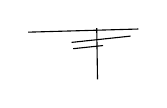
\begin{tikzpicture}[x=1cm,y=1cm]\draw (0,0.6)--(1.4,0.64);\draw (0.55,0.47)--(1.30,0.55);\draw (0.57,0.39)--(0.95,0.43);\draw (0.88,0)--(0.87,0.65);\end{tikzpicture}}
\end{center}
On aimerait prouver un th. d'unicité (\unsure{on a déjà l'existence}$\ldots$)

Les $C_*^{**}$ ayant les structures précisées (au besoin \unsure{on oublie d'abord} la structure p.d.) et satisfaisant
\margin{118}

\scanpage{120}
\begin{tabular}{c}
COLLÈGE\\DE\\FRANCE\\---
\end{tabular}
\hfill\begin{tabular}{l}\textit{Paris, le}\\xxxxx\end{tabular}\quad Massy le 14.9.1971

Cher Monsieur Poncet,

Je viens d'avoir connaissance de deux ennuis sérieux avec la \unsure{machine|mechine} Hermès 3000 que vous m'aviez livrée en juin: le margeur gauche ne fonctionne plus, et l'enroulement du ruban est défectueux, ne permettant d'utiliser qu'une partie du ruban et obligeant de ce fait à des manipulations supplémentaires fort gênantes. Ces ennuis se présentent alors que la machine a encore à peine servi (une trentaine de pages de texte environ), et il est clair que la qualité des machines Hermès 3000 a considérablement baissée depuis une dizaine d'années (j'ai une machine avec laquelle je n'ai eu aucun ennui depuis cette période). C'est pourquoi je me vois dans l'obligation \inserted{d'annuler} la commande d'une autre machine Hermès 3000 que je vous avais faite vers la fin du mois d'août (lettre datée erronément du 1.6.1971 ...), préférant m'adresser à une marque de machine portative qui ne m'exposera pas à des contretemps \unsure{continuels}
Au cas où à la réception de la présente lettre, la livraison aurait déjà été faite, je vous serais obligé de la reprendre au Collège de France. Je vous renvoie ci-jointsfacture et bon de garantie relatifs à cette commande.

Veuillez agréer, cher Monsieur, l'expression de ma considération la plus distinguée
\margin{119}

\scanpage{121}
aux conditions supplémentaires techniques énoncées (être une ``quasi'' résolution de $S_k$, et être ``quasi-flasque'' $\ldots$)

On note que les hom. dans \deleted{\unsure{cette}} la catégorie des objets \inserted{$C_*^{**}$} envisagés sont déjà des ``quasi-iso'' (pour $\tau_\infty$) - il y a lieu de passer à la cat. des fractions en \deleted{les} rendant inversibles tous ces hom., i.e. le \uline{groupoïde engendré} par la catégorie \uline{envisagée}. On aimerait donc prouver que ce groupoïde est connexe et simplement connexe ?
[\uline{NB} rappelons \unsure{que c'est en un} \uline{langage pr} \inserted{\unsure{en dehors}} $S_k=k\{T\}$ \unsure{bien entendu plus qu'il y ait calcul de fractions à gauche}]

Cela signifie donc

\uline{Conj.?} a) Si $C_*^{**}$ et $C'_*{}^{**}$ sont des théories admissibles, $\exists$ théorie admissible $C''_*{}^{**}$ et hom
\[
\diagram{\begin{tikzcd}
&C_*^{**}\\
C''_*{}^{**}\arrow[ur]\arrow[dr,no head]\\
&C'_*{}^{**}
\end{tikzcd}}
\]
\margin{\figure{\begin{tikzpicture}[x=1cm,y=1cm]\draw (0,0)--(0,4);\node at (-0.6,2.9) {\Huge ?};\end{tikzpicture}}}
b) Si on a deux hom
\[
\diagram{\begin{tikzcd}
C'_*{}^{**}\arrow[r,shift left=0.7ex]\arrow[r,shift right=0.7ex,no head]&C_*^{**}
\end{tikzcd}}
\]
$\exists$ hom
\[
\diagram{\begin{tikzcd}
C''_*{}^{**}\arrow[r,no head]&C'_*{}^{**}
\end{tikzcd}}
\]
qui ``égalise''.
\margin{\unsure{il y aurait} plus de chances avec calcul de fractions à droite ???}
\margin{\figure{\begin{tikzpicture}[x=1cm,y=1cm]\draw (0,0)--(1.1,3.6);\end{tikzpicture}}}
\margin{120}

\scanpage{123}
\begin{flushright}
\fbox{\parbox{.53\linewidth}{Complexes de \uline{données} de De Rham\\ à p.d.}}
\end{flushright}
\begin{minipage}[t]{.43\linewidth}
Soient

$k$ anneau comm.

\deleted{\illegible{1}} \textcircled{$S$} une $k$-coalgèbre \inserted{ass. unitaire comm.}

\deleted{\illegible{1}}

\textcircled{$\bar S$} une sous-$k$-coalgèbre \inserted{ass. unit. comm.}
\[
\diagram{\begin{tikzcd}[row sep=large]
\bar S \arrow[d,Leftrightarrow]\\
S^+
\end{tikzcd}}
\]
\textcircled{$S^+$} $=S/\bar S$ le $k$-module quotient

[c'est une coalgèbre ass. comm. mais pas unitaire]

\textcircled{$\gamma_*$} un système de copuissances divisées sur $(S,S^+)$
\end{minipage}\hfill
\begin{minipage}[t]{.54\linewidth}
\[
\boxed{S\longrightarrow S\otimes_k S}
\]
[d'où \inserted{$V_k(S):$} $k'\longmapsto S^{k'}=\operatorname{Hom}_k(S,k')$ est un foncteur : \unsure{$\mathcal O_k$} dans les anneaux \unsure{commut.} \unsure{autrement dit} une $\mathcal O_k$-Alg. ass. uni comm.

[d'où \inserted{$V_k(\bar S):$} $k'\longmapsto\bar S^{k'}=\operatorname{Hom}_k(\bar S,k')$ est une $\mathcal O_k$-alg. ass. unit. comm. et $S^{k'}\longrightarrow\bar S^{k'}$ est un hom. de $k'$-Alg. ass. unit. comm. \inserted{i.e. $V_k(S)\longrightarrow V_k(\bar S)$ hom. de $\mathcal O_k$-algs.}

[$S^{+\,k'}\simeq\operatorname{Ker}(S^{k'}\longrightarrow\bar S^{k'})\subset S^{k'}$ est un idéal de $S^{k'}$, donc $V_k(S^+)\overset{\mathrm{dfn}}=V_k(S)^+$ est un Idéal de $V_k(S)$]

[d'où on a sur $V_k(\unsure{S^+|\bar S})=V_k(S)^+$ un syst. de puiss. divisées
\[
\gamma_i:V_k(S^+)\longrightarrow V_k(S^+)\qquad i\geq1
\]
définis par des hom de $k$-alg
\[
\gamma_i^*:\operatorname{Sym}_k(S^+)\longrightarrow\operatorname{Sym}_k^{\unsure{*}}(S^+)
\]
\deleted{\unsure{qui}} \unsure{des hom. de $k$-m}
\[
\gamma_i^*:S^+\longrightarrow\operatorname{Sym}_k^{\unsure{*}}(S^+)
\]
(qui, en vertu des axiomes sont en fait
\[
\boxed{\gamma_i^*:S^+\longrightarrow\operatorname{Sym}_k^i(S^+)\quad(i\geq1)}
\]
avec des axiomes dessus
\end{minipage}

\[
 t:S^+\longrightarrow k\quad\text{un $k$-hom.}\qquad
\text{i.e. }t\in V_k(S^+)(k)=V_k(S)^+(k)
\]
\figure{\begin{tikzpicture}[x=1cm,y=1cm]\draw (0,.65) .. controls (1,.85) and (.6,-.1) .. (1.6,-.1)--(2.05,-.1);\end{tikzpicture}}

Alors on définit un objet \unsure{simplicial} dans la cat. des foncteurs
\[
(k\text{-alg comm})\longrightarrow
\left(\begin{array}{l}\text{algèbres graduées alternées différentielles}\\
\text{(diff. de degré $+1$) à}\ \inserted{\text{avec idéaux à}}\\
\text{puiss. divisées (}\end{array}\right.
\]
et $\simeq$ dans la cat des \deleted{foncteurs} schémas affines \deleted{\illegible{1}} en algèbres graduées alternées différentielles (diff. de degré $+1$) avec Idéal \inserted{\uline{homogène}} à p. div. (qui est un schéma affine), les puiss. div. étant compatibles avec graduation et avec différentielle

\margin{122}

\scanpage{124}
\begin{center}- \mspage{120} -\end{center}\margin{IX}

un accouplement
\[
(*)\qquad v_\ell^{K'}:\underline M_K\otimes\underline M'_K\longrightarrow\mathbb Z_{\ell K}.
\]
Ce dernier à priori dépend du choix de $K'$, mais il résulte de (10.4.3) ci-dessous que l'accouplement
\[
(9.7.1)\qquad u_\ell:\underline M_K\otimes\underline M'_K\longrightarrow\mathbb Q_{\ell K}
\]
donné par
\[
u_\ell=(1/e(S'/S))\,v_\ell^{K'}
\]
n'en dépend pas, où $e(S'/S)=\operatorname{long}(V'/\underline mV')$. On pourra appeler encore (9.7.1) l'\uline{accouplement de monodromie} pour le schéma abélien $A_K$ sur $K$ et le nombre premier $\ell$ envisagé, puisque dans le cas où $A_K$ lui-même a réduction semi-stable, il coïncide évidemment avec la restriction à $\eta$ de l'accouplement de monodromie (9.1.2). Il résulte de 10.4 plus bas que cet accouplement est en fait toujours à valeurs dans $\mathbb Q_K$, et est indépendant de $\ell$.

On peut se demander s'il est à valeurs dans $\mathbb Z_K$, ce qui revient à dire que (9.7.1) est à valeurs dans $\mathbb Z_{\ell K}$ pour tout nombre premier $\ell$. C'est le cas du moins si $A_K$ est une courbe elliptique, le seul cas qui demande une vérification étant alors celui où $\underline M_K\simeq\underline M'_K$ est de rang 1, de sorte que $\underline M_K\otimes\underline M'_K$ est canoniquement isomorphe à $\mathbb Z_K$, et que l'accouplement de monodromie (9.7.1) peut s'interpréter simplement comme un nombre rationnel ordinaire. On trouve grâce aux résultats de NERON [19] que celui-ci est égal à $v(j)$, $j$ étant l'invariant absolu de $A_K$ et $v$ la valuation normalisée de $K$.

\margin{438}\margin{438}\margin{123}

\scanpage{125}
\[
\underbrace{A_*^*(\unsure{S},S^+,\gamma_*,t)}_{\begin{array}{l}\text{schéma affine}\\\text{en alg. graduées}\\\text{(alternées différentielles}\\\text{($d$ de degré 1) avec idéal hom.}\\\text{à p.d. (\unsure{si on veut})}\end{array}}(k')
=A_*^*\left(\underset{\substack{\Vert\\V_k(S)(k')}}{S^{k'}},\underset{\substack{\Vert\\V_k(S^+)(k')}}{(S^{k'})^+},\gamma_*^{k'},t^{k'}\right)
\]
On a
\[
 A_*(S,S^+,\gamma_*,t)(k')(\bar I)\simeq
 \widehat\Gamma^{\unsure{'|*}}_{\unsure{S_*^{k'}}}\{\{k'^I\}\}\otimes_{k'}\Lambda^*(k'^I/k')\big/\begin{array}{l}\text{idéal p.d.}\\\text{engendré}\\\text{par }\sum X_i-t\end{array}
\]
\[
\begin{aligned}
 A_n(S,S^+,\gamma_*,t)(k')
 &\simeq\deleted{\unsure{k}}S^{k'}\{\{X_0,\ldots,\overset{\inserted{\widehat\Gamma}}{X_n}\}\}[dX_0,\ldots,dX_n]/(\textstyle\sum X_i-t,\sum dX_i)_{\unsure{\mathrm{pd}}}\\
 &\simeq S^{k'}\{\{X_0,\ldots,X_{n-1}\}\}[dX_0,\ldots,dX_{n-1}]\\
 &\underset{\substack{\text{comme}\\\text{foncteur en }k'}}\simeq
 \deleted{\unsure{k}}(S^{k'})^{\mathbb N^n\times\unsure{\mathcal P|\mathfrak P}([0,n-1])}\\
 &\underset{\substack{\text{comme foncteur en}\\k'}}\simeq
 \operatorname{Hom}_k(S,k')^{\mathbb N^n\times\mathcal P([0,n-1])}\\
 &\underset{\cdots}\simeq\operatorname{Hom}_k\bigl(S^{(\mathbb N^n\times\mathcal P([0,\unsure{n-1|1}]))},k'\bigr)\\
 &=V\bigl(\underbrace{S^{(\mathbb N^n\times\mathcal P([0,n-1]))}}\bigr)(k')\\
 &=V\bigl(S\otimes_k k[Y_0,\ldots,Y_{n-1}]\otimes_k\Lambda^*(y_0,\ldots,y_{n-1})\bigr)(\unsure{k'|k''})
\end{aligned}
\]
\figure{\begin{tikzpicture}[x=1cm,y=1cm]\draw[->] (1,.8)--(.2,0);\end{tikzpicture}}
\margin{ens des parties}
\figure{\begin{tikzpicture}[x=1cm,y=1cm]\draw[->] (0,1) .. controls (.1,.5) and (.4,.2) .. (1,0);\end{tikzpicture}}
\[
 A_n(S,S^+,\gamma_*,t)(k')/A_n(\quad)(k')^+\simeq
 S^{k'}/(S^{k'})^+\unsure{\leftarrow}\bar S^{k'}
\]
\[
\diagram{\begin{tikzcd}[column sep=large,row sep=large]
 A_n(\qquad)(k') \arrow[r] \arrow[d,phantom,"\Vert"] & \bar S^{k'}=V(\bar S)(k')\\
 V(S\otimes_k k[Y_0,\ldots,Y_{n-1}]\otimes_k\Lambda^{\unsure{*}}(y_0,\ldots,y_{n-1}))(k') \arrow[r] & V(\bar S)(k')
\end{tikzcd}}
\]
\[
\diagram{\begin{tikzcd}[column sep=huge,row sep=large]
 S\otimes_k k[Y_0,\ldots,Y_{n-1}]\otimes_k\Lambda^{\unsure{*}}(y_0,\ldots,y_{n-1}) & \bar S \arrow[l] \arrow[d,hook]\\
 & S \arrow[ul,hook']
\end{tikzcd}}
\]
On voit donc, posant
\[
 A_*^n(S,S^+,\gamma_*,t)=S\otimes_k k[Y_0,\ldots,Y_{n-1}]\otimes_k\Lambda^*(y_0,\ldots,y_{n-1})
\]
\margin{124}

\scanpage{126}
\begin{center}- \mspage{119}\end{center}\margin{IX}

Comme extension panachée $X_\eta$ de $E_\eta$ par $F_\eta$, on prendra
\[
(9.6.2)\qquad X_\eta=T_\ell(A_K)=X_\eta^0\supset X_\eta^1=T_\ell(A_K)^f\supset X_\eta^2=T_\ell(A_K)^t\supset0.
\]
L'isomorphisme d'extensions de $R_\eta$ par $P_\eta$
\[
 X_\eta^1\simeq F_\eta
\]
est clair. L'isomorphisme d'extensions de $Q$ par $R$ :
\[
 X_\eta/X_\eta^2\simeq F_\eta=D(F'_\eta)
\]
est clair grâce au théorème d'orthogonalité 5.2.

Nous disposons donc des données requises pour définir un accouplement (9.5.6), qui ici (comme $Q^*=\underline M'_\ell$) prend la forme (9.1.2). Le fait que cette définition soit compatible avec celle de 9.2 résulte de 9.5.8. Les considérations de 5.3 montrent d'autre part, sous réserve de la validité du théorème de TATE [33] (donc en tous cas dans le cas où car $K=0$) que l'accouplement en question peut se décrire en termes du seul $\ell$-pro-groupe de Barsotti-Tate $X_\eta=T_\ell(A_K)$ sur $S$ (puisque sa filtration en trois crans, et les extensions $F$ et $E$ qui prolongent $X_\eta^1$ et $X_\eta/X_\eta^2$, peuvent se définir canoniquement en termes du seul pro-$\ell$-groupe $X=T_\ell(A_K)$.
\figure{\begin{tikzpicture}[x=1cm,y=1cm]\draw (0,0)--(.12,.1);\draw (0,.1)--(.12,0);\end{tikzpicture}}

\uline{Remarque} 9.7. Ne supposons plus nécessairement que $A_K$ ait réduction semi-stable sur le trait hensélien $S$, et soit $K'$ une extension galoisienne finie de $K$ telle que $A_{K'}$ ait réduction semi-stable sur le normalisé $S'$ de $S$ dans $K'$ (3.6). Avec les notations de (8.1.8), on définit alors, par descente galoisienne à partir de l'accouplement de monodromie pour $A_{K'}$,

\margin{\unsure{437}}\margin{437}\margin{125}

\scanpage{127}
a) Chacun des $A^{\unsure{n}}(-)$ est muni d'une structure de $k$-coalgèbre \inserted{(alternée)} graduée codifférentielle (codifférentielle de degré $-1$), avec \unsure{l'immersion|l'inclusion} $\bar S\hookrightarrow A^n(-)$ qui est compatible avec tout (prenant sur $\bar S$ la graduation nulle, et la différentielle nulle), et \deleted{une}\inserted{un} syst. de copuissances divisées sur
\[
 A^{\unsure{n}}(\quad)^+=A^n(\quad)/\bar S,
\]
compatibles avec graduation et différentielle.

b) Pour $n$ variable, les $A^n(\quad)$ forment un objet $\frac12$\inserted{co}simplicial (et $=$ simplicial) $A^*(S,S^+,\gamma_*,t)$ dans la cat. des \inserted{objets, avec ces structures} (coalg\ldots) \unsure{décrite dans a)}.

c) On reconstitue $A_*(S,S^+,\gamma_*,t)$ \inserted{$=k'\longmapsto A_*(S,\gamma_*,t)(k')$} avec toutes ses structures à l'aide des $A^*(S,S^+,\gamma_*,t)$, comme
\[
 A_*(S,S^+,\gamma_*,t)=V_k\bigl(A^*(S,S^+,\gamma_*,t)\bigr)
\]

d) Soit $X$ un ens. $\frac12$ simplicial, considérons
\[
\begin{aligned}
 k'&\longmapsto\operatorname{Hom}(X,A_*(-)(k'))
 \overset{\mathrm{dfn}}=C^*_{\mathrm{DR}}(X;S^{k'},(S^{k'})^+,\gamma_*^{\unsure{k'}},\unsure{t^{k'}|t})\\
 &\simeq\varprojlim_{\sigma\text{ ds }\Delta/X}\operatorname{Hom}(\sigma,A_*(\quad)(k'))\\
 &\simeq\varprojlim_{\sigma\text{ ds }\Delta/X}\underbrace{A_{\dim\sigma}(\quad)(k')}_{\operatorname{Hom}_k(A^{\dim\sigma}_{\deleted{\unsure{\dim\sigma}}}(-),k')}\\
 &\simeq\operatorname{Hom}_k\left(\varinjlim_{\sigma\text{ ds }\Delta/X} A^{\dim\sigma}_{\deleted{\unsure{\dim}}}(-),k'\right)\\
 &\simeq\operatorname{Hom}_k\bigl(C_*^{\mathrm{DR}}(X;S,S^+,\gamma_*,t),k'\bigr)
\end{aligned}
\]
\margin{$\Delta$ : cat. des simplexes types $(\Delta_i)_{i\geq0}$\quad $\Delta_i=[0,i]$}
\figure{\begin{tikzpicture}[x=1cm,y=1cm]\draw[->] (0,.8) .. controls (-.15,.2) and (-.05,.15) .. (.2,.2);\end{tikzpicture}}
\margin{126}

\scanpage{128}
\begin{center}- \mspage{118} -\end{center}\margin{IX}

de type fini. On constate alors que l'homomorphisme (9.5.6) est l'homomorphisme canonique qui exprime l'action du sous-groupe d'inertie $I\subset\pi$ sur $X_\eta(\bar K)$, défini par la méthode de 9.2. Pour le vérifier, on se ramène immédiatement à la situation de 9.4, en y supposant que $n$ est égal à une puissance de $\ell$, et que $R$ est un $\Lambda$-Module localement constant (tout comme $Q$ et $P$), de sorte qu'il en est également de même de $E$, $F$ et de $X_\eta$. La vérification de l'identité des deux définitions est alors laissée au lecteur.

9.6. Nous sommes maintenant en mesure de définir l'accouplement canonique annoncé (9.1.2), sans restriction sur $\ell$, de telle façon que pour $\ell\neq p$ cette définition coïncide avec celle donnée dans 9.2. Pour ceci, on applique les considérations de 9.5 à la situation suivante :
\[
(9.6.1)\quad\left\{\begin{array}{l}
P=T_\ell(A^0)^t=\check{\underline M}'_\ell(1),\quad Q=M_\ell,\quad R=T_\ell(A^0)^f/T_\ell(A^0)^t,\\[2em]
F=T_\ell(A^0)^f,\quad E=D(F')=D(T_\ell(A'^0)^f),
\end{array}\right.
\]
où dans la dernière formule $D$ désigne le dual de Cartier au sens des pro-$\ell$-groupes de Barsotti-Tate, i.e $D(Y)$ est le système \uline{projectif} des $D(Y(n))$, pour les morphismes de transition habituels. La structure de $F$ comme extension de $R$ par $P$ est claire. On a de même sur $F'=T_\ell(A'^0)^f$ une structure d'extension de $R'$ par $P'=T_\ell(A'^0)^t=\check{\underline M}_\ell(1)$. Appliquant la dualité de Cartier, on en conclut que $E=D(F')$ est muni d'une structure d'extension de $D(P')=M_\ell$ par $D(R')$. Or $D(R')$ est canoniquement isomorphe à $R$ en vertu de 5.5 (prouvé dans 7.4.6), ce qui précise la structure de $E$ comme extension de $Q$ par $R$.

\margin{\unsure{436|426}}\margin{436}\margin{127}

\scanpage{129}
\unsure{où}
\[
\boxed{C_*^{\mathrm{DR}}(X;S,S^+,\gamma_*,t)\overset{\mathrm{dfn}}=\varinjlim_{\sigma\text{ ds }\Delta/X} A^{\dim\sigma}(S,S^+,\gamma_*,t)}
\]
Ici $C_*^{\mathrm{DR}}(X;S,S^+,\gamma_*,t)$ est une $k$-coalgèbre graduée (alternée) codiff. (codiff. de degré $-1$), \deleted{à copuissances}\inserted{avec un} \deleted{divisées} \inserted{hom} \deleted{\unsure{k}} $\bar S\longrightarrow C_*^{\mathrm{DR}}(X,-)$ \inserted{pour toutes structures} (pas néc injectif p. ex. si $X=\varnothing$ $C_*^{\mathrm{DR}}(X,-)=0$ \unsure{--}) et des puiss. divisées sur \deleted{\unsure{id}} $C_*^{\mathrm{DR}}(X,-)_+=\operatorname{Coker}(\bar S\longrightarrow C_*^{\mathrm{DR}}(X,-))$. Il est covariant en $X$ avec ttes ses structures, et $C^*_{\mathrm{DR}}(X,S^{k'},-)$ est contravariant en $X$. \deleted{\unsure{Il est covariant en}}

\margin{$X\longmapsto C_*^{\mathrm{DR}}(X,-)$ \unsure{dépend de $X$ en commutant} aux $\varinjlim$ quelconques (non seult filtrantes)}

\textcircled{e)} Si $(S,S^+,\gamma_*,t)$ varie sur $k$, $(S^{k'},S^{+\,k'},\gamma_*^{k'},t^{k'})$ en dépend de façon contravariante, donc $C^*_{\mathrm{DR}}(X;S^{k'},S^{+\,k'},\gamma_*^{k'},t^{k'})$ aussi
\[
 \operatorname{Hom}(\unsure{\text{``}|=}C_*^{\mathrm{DR}}(X,-),k'),
\]
et $C_*^{\mathrm{DR}}(X;S,S^+,\gamma_*,t)$ dépend de façon covariante de $(S,S^+,\gamma_*,t)$, ce qui est aussi évident sur l'écriture plus haut $C_*^{\mathrm{DR}}(X,-)=\varinjlim\ldots$, compte tenu que $A^*(S,S^+,\gamma_*,t)$ est covariant en $(S,S^+,\gamma_*,t)$. De plus, \deleted{il} comme foncteur en $(S,S^+,\gamma_*,t)$, il commute aux $\varinjlim$ quelc.

Commutation à l'extension de l'anneau de base.

f) Supposons que la coalgèbre $S$ soit graduée (structure de coalgèbre et graduation compatibles) que $\bar S$ soit \unsure{itou}, $\bar S\longrightarrow S$ compatible avec, les p.d. sur $S^+$ compatibles avec graduation, et
\[
 t:S^+\longrightarrow k\quad\inserted{\text{hom}}\ \text{de degré }\delta.
\]
Alors \deleted{\unsure{les}\ \illegible{1}} \inserted{$\forall k'$}, $(S^{k'},S^{+\,k'},\gamma_*^{k'},\unsure{t^{k'}})$
\margin{128}

\scanpage{130}
\begin{center}- \mspage{117} -\end{center}\margin{IX}

Pour tout entier $n$, l'homomorphisme correspondant $X(n)\longrightarrow Q(n)$, étant surjectif sur les fibres génériques, est surjectif ; comme $Q(n)$ est étale sur $\unsure{n|\eta}$, donc $X(n)\longrightarrow Q(n)$ est plat, il s'ensuit que c'est un épimorphisme. Donc $X\longrightarrow Q$ \uline{est un épimorphisme composant par composant}. Si donc $\bar F$ désigne le noyau de $X\longrightarrow Q$, il s'ensuit que $\bar F$ est un groupe de Barsotti-Tate et $X$ est une extension de $Q$ par $\bar F$. D'ailleurs l'isomorphisme $F_\eta\overset\sim\longrightarrow\bar F_\eta$ se prolonge, par le théorème de TATE, en un isomorphisme $F\simeq\bar F$. Par suite, $X$ apparaît comme une extension de $Q$ par $F$. Considérons alors le quotient $\bar E=X/P$, on voit encore, par application du théorème de TATE, qu'on a un isomorphisme $E\simeq\bar E$. Il s'ensuit que $X$ est une extension panachée de $E$ par $F$ prolongeant l'extension panachée $X_\eta$, cqfd.

\uline{Remarques} 9.5.6.4. a) Bien entendu, la dernière assertion de 9.5.6 devrait être valable sans restriction sur $K$, puisqu'il devrait en être ainsi du théorème de Tate invoqué.

b) On peut donner une autre démonstration du critère de bonne réduction 5.10, en se ramenant comme dans 5.10 au cas où $A_K$ est à réduction semi-stable, et en appliquant alors 9.5.6 à $T_\ell(A_K)$ considérée comme extension panachée (cf. 9.6), qui implique $u_\ell=0$, et utilisant 11.6.2 a) plus bas qui implique que l'on a $T_\ell(A_K)^t=0$.

9.5.8. Lorsque $\ell\neq p$, les groupes de Barsotti-Tate envisagés sur $S$ resp. sur $K$ s'interprètent simplement en termes de faisceaux $\ell$-adiques constants tordus sur $S$, ou de façon équivalente, en termes de représentations de $\pi_{\unsure{0|o}}=\operatorname{Gal}(\bar k/k)$ resp. de $\pi=\operatorname{Gal}(\bar K/K)$ sur des $\mathbb Z_\ell$-modules libres

\margin{435}\margin{129}

\scanpage{131}
est une alg. \deleted{à p.div.} \uline{graduée}, avec idéal $(S^{k'})^+$ \uline{hom.} à p.div. compatibles avec graduation, et $t^{k'}$ est un élém de degré $\delta$ \unsure{du dit}.

Alors les
\[
 A_n(\qquad)(k')=S^{k'}\{\{X_0,\ldots,X_n\}\}[dX_0,\ldots,dX_n]/(\textstyle\sum X_i-t,\sum dX_i)_{\mathrm{pd}}
\]
\inserted{une alg.} est \uline{bigraduée}, par le degré extérieur déjà envisagé ($2^{\text{ième}}$ degré) \inserted{(nul sur $S^{k'}$)}, et le degré total défini par
\[
\left\{\begin{array}{l}
\deg\operatorname{tot}X_r=\deg\operatorname{tot}dX_r=\delta\quad\deleted{\unsure{\deg}}\\
\deg\operatorname{tot}X_r^{(i)}=\unsure{\delta i|\delta};\quad\deg\operatorname{tot}_A\lambda=\deg\operatorname{tot}_{S^{k'}}\lambda\quad\big|\ \lambda\in S^{k'}
\end{array}\right.
\]
La diff. \deleted{\unsure{affecte}} \unsure{respecte} le degré total, $A_n(\quad)(k')$ est pour le degré tot une \uline{alg.} graduée sur $S^{k'}$ graduée commutative diff.; les puiss. divisées sont compatibles avec deux degrés.

Cette structure supplémentaire (deg tot.) est \deleted{\unsure{encore}} fonctorielle en $k'$, donc passe à $A^*(S,S^+,\gamma^*,t)$. Elle passe par suite aux $C_*^{\mathrm{DR}}(X;S,S^+,\gamma^*,t)$, et on retrouve la structure déjà connue de $C^*_{\mathrm{DR}}(X;S^{k'},(S^{k'})^+,\gamma_*^{k'},t^{k'})$ en prenant le $\operatorname{Hom}_k$ du \deleted{\unsure{$C$}} $C_*^{\mathrm{DR}}(X;S,S^+,\gamma^*,t)$ dans $k'$.

g) On prendra maintenant, \unsure{pour}
\[
\begin{array}{ll}
S=\deleted{\unsure{S}}S_k=k[u]&\text{donc }S^{k'}=k'\{\{T\}\}\\
\bar S=\bar S_k=k&\text{donc }\bar S^{k'}=k'
\end{array}
\]
\inserted{avec structure de coalg. \unsure{ordinaire}, \deleted{\illegible{1}} \unsure{sur $S_k$ la structure d'anneau}}
\[
\begin{array}{ll}
\bar S\longrightarrow S\quad\text{l'inclusion}&\text{donc }S^{k'}\longrightarrow\bar S^{k'}\quad\text{l'augm. canonique}\\
k\longrightarrow k[u]&k'\{\{T\}\}\longrightarrow k'
\end{array}
\]
\[
 \unsure{S^+}=k[u]/k\simeq k[u]^+
\]
\margin{130}

\scanpage{132}
\margin{131}
\begin{center}- \mspage{116} -\end{center}\margin{IX}

\uline{dans la catégorie des extensions panachées de} $E_\eta$ \uline{par} $F_\eta$. \uline{Pour tout groupe de Barsotti-Tate extension panachée} $X_\eta$ \uline{de} $E_\eta$ \uline{par} $F_\eta$, \uline{on considère l'accouplement correspondant}
\[
(9.5.6.2)\qquad Q_0\otimes Q_0^*\longrightarrow\mathbb Z_{\ell S},
\]
\uline{induit par l'accouplement du type} (9.5.5) \uline{défini sur le} hensélisé \uline{de} $S$. \uline{Ceci posé}, \uline{le foncteur} (9.5.6.1) \uline{est pleinement fidèle}, \uline{et son image essentielle est formée des groupes de Barsotti-Tate} $X_\eta$ \uline{extensions panachées de} $E_\eta$ \uline{par} $F_\eta$ \uline{telles que l'accouplement} (9.5.6.2) \uline{correspondant soit nul}. \uline{De plus}, \uline{lorsque} car.$K=0$ (\uline{de sorte qu'on peut appliquer le théorème de TATE} [33 th. 4]), \uline{alors} $X_\eta$ \uline{appartient à l'image essentielle si et seulement si} $X_\eta$ \uline{se prolonge en un groupe de Barsotti-Tate sur} $S$.

9.5.6.3. Nous laissons au lecteur le soin d'étendre cet énoncé au cas où on suppose seulement que $S$ est un schéma noethérien régulier connexe de dimension 1.

La première assertion de 9.5.6 est une conséquence immédiate de 9.4.6, appliqué aux composants des groupes de Barsotti-Tate envisagés. Il reste à prouver que si un groupe de Barsotti-Tate $X_\eta$, extension panachée de $E_\eta$ par $F_\eta$, se prolonge en un groupe de Barsotti-Tate $X_\eta$ sur $S$, il se prolonge aussi comme extension panachée. Or en vertu du théorème de TATE [33], l'homomorphisme $X_\eta\longrightarrow Q_\eta$ se prolonge de façon unique en un homomorphisme
\[
 X\longrightarrow Q.
\]
\margin{\unsure{434}}\margin{434}

\scanpage{133}
On prend syst. de copuiss. divisées sur $k[u]^+=S^+$ correspondant à celles \deleted{de}\inserted{canoniques} de $k'\{\{T\}\}^+$.

On prend $t\in k\{\{T\}\}$ donné par $t=T$, i.e.
\[
 t(u^n)=\left\{\begin{array}{ll}1&\text{si }n=1\\0&\text{si }n\neq1\end{array}\right.
\]
On a donc ici
\[
\begin{aligned}
 A_*(S,S^+,\gamma^{\unsure{*}},t)(k')
 &\simeq A_*(S^{k'},S^{+\,k'},\gamma_*^{k'},t^{k'})\\
 &\simeq A_*(k'\{\{T\}\},k'\{\{T\}\}^+,\gamma^{k'},T)\\
 &\simeq A_*(k')^\wedge
\end{aligned}
\]
On pose simplement
\[
 \deleted{\unsure{A_k^*}}\quad A_{k\unsure{*}}^*=A_k^*(S_k,\bar S_k,\gamma_k^*,t_k)
\]
de sorte que
\[
 A_*(k')^\wedge\simeq\operatorname{Hom}_k(A_k^*,k')
\]
``avec toutes les structures''. Notons qu'ici on est dans le cas où $S$, $\bar S$ et $\bar S\longrightarrow S$ sont gradués (graduation ordinaire de $k[u]$, correspondant à la graduation naturelle sur les $k'\{\{T\}\}$) et $t=T$ de \inserted{hom} degré 1, donc \deleted{$\unsure{A_k^*}$} $A_k^*$ admet une bigraduation. Celle-ci passe aux \deleted{\unsure{$C_*^*$}}
\[
 \deleted{C_*^{\mathrm{DR}}(X;k)}
\]
\[
 C_*^{\mathrm{DRpd}}(X,k)\overset{\mathrm{dfn}}\simeq C_*^{\mathrm{DR}}(X,k[u];k[u]^+,\gamma_k^*,t_k)
\]
\inserted{(avec les autres)}, et redonne par $\operatorname{Hom}_k(C_*^{\mathrm{DRpd}}(X,k),k')$ les structures connues (y compris bigraduation) sur le complexe de cochaînes de De Rham $C^*_{\mathrm{DRpd}}(X,k')$.

En fait tous les $C_*^{\mathrm{DRpd}}(X,k)$ ($k$ variable)
\margin{132}

\scanpage{134}
\begin{center}- \mspage{115} -\end{center}\margin{IX}

enfin donnée sur $\eta$ un pro-$\ell$-groupe de Barsotti-Tate $X_\eta$ qui soit \uline{extension panachée} de $E_\eta$ par $F_\eta$, par quoi nous entendons qu'il est muni d'une filtration en trois crans (en tant que pro-$\ell$-groupe de Barsotti-Tate), donnant lieu à des extensions partielles munies d'isomorphismes avec $E_\eta$ et $F_\eta$ respectivement. Il s'ensuit que pour tout $n$, $X_\eta(n)$ est muni d'une structure d'extension panachée de $E(n)_\eta$ par $F(n)_\eta$. Nous pouvons lui faire correspondre alors un accouplement du type (9.4.1) :
\[
(9.5.4)\qquad c(X(n)_\eta):Q(n)\otimes Q^*(n)\longrightarrow\Lambda_n=\mathbb Z/\ell^{n+1}\mathbb Z,
\]
où les $Q^*(n)$ sont les groupes finis étales sur $S$ définis par
\[
P(n)\simeq D(Q^*(n)),\quad\text{i.e.}\quad Q^*(n)=D(P(n)),
\]
$D$ désignant encore la dualité de Cartier. Les $Q^*(n)$ forment un pro-$\ell$-groupe de façon évidente, soit $Q^*$. Nous laissons au lecteur le soin de vérifier que pour $n$ variable, les homomorphismes (9.5.4) définissent un homomorphisme de systèmes projectifs, i.e. un homomorphisme de faisceaux $\ell$-adiques constants tordus sur $S$ :
\[
(9.5.5)\qquad c(X_\eta):Q\otimes Q^*\longrightarrow\mathbb Z_{\ell S}.
\]

Signalons en passant le résultat suivant (qui ne sera pas utilisé dans la suite) :

\uline{Proposition} 9.5.6. \uline{Les données} $P,Q,R,E,F$ \uline{sont les mêmes que ci-dessus}, \uline{sauf qu'il est inutile de supposer le trait} $S$ \uline{hensélien}. \uline{On considère le foncteur}
\[
(9.5.6.1)\qquad X\longmapsto X_\eta
\]
\uline{de la catégorie des extensions panachées de Barsotti-Tate de} $E$ \uline{par} $F$

\margin{\unsure{433|432}}\margin{433}\margin{133}

\scanpage{135}
\unsure{se déduisent de}
\[
 C_*^{DRpd}(X)\overset{\mathrm{dfn}}=C_*^{DRpd}(X;\mathbb Z)
\]
\unsure{par la formule}
\[
 C_*^{DRpd}(X,k)\simeq C_*^{DRpd}(X)\otimes_{\mathbb Z}k,
\]
\unsure{et on a de même}
\[
 C^*_{DRpd}(X,k)\simeq\unsure{\operatorname{Hom}}(C_*^{DRpd}(X,k))
\]

On définit de même, pour \unsure{tt} groupe \unsure{abélien} $M$ et \unsure{fonctoriellement} en $M$
\[
\begin{aligned}
 C_*^{DRpd}(X;M)&\overset{\mathrm{dfn}}=C_*^{DRpd}(X)\otimes_{\mathbb Z}M\\
 C^*_{DRpd}(X,M)&\overset{\mathrm{dfn}}=\operatorname{Hom}(C_*^{DRpd}(X),M)
\end{aligned}
\]
et les structures sur $C_*^{DRpd}(X)$ \unsure{impliquent} une \unsure{foule} de structures \unsure{multiplicatives} pour \unsure{ces} foncteurs en $M$ \unsure{\ldots}

\margin{134}

\scanpage{136}
\begin{center}- \mspage{114} -\end{center}\margin{IX}

qui est injective (puisque la suite exacte $0\longrightarrow V^*\longrightarrow K^*\longrightarrow\mathbb Z\longrightarrow0$ est scindée), donc elle est injective, ce qui implique (grâce au \unsure{cor. thé.|corthé} 9.3) que si $X_\eta$ et $Y_\eta$ sont isomorphes, il en est de même de $X$ et de $Y$. On gagne donc par a).

Evidemment a) et b) impliquent que le foncteur $X\longmapsto X_\eta$ est \uline{pleinement} fidèle.

c) Soit $X_\eta$ une extension panachée sur $\eta$, prouvons qu'elle se prolonge à $S$ si et seulement si les accouplements (9.4.6.2) sont nuls. Ici encore, l'unicité déjà prouvée montre que la question est locale pour la topologie étale, ce qui nous ramène encore au cas $S$ strictement local. Alors la conclusion est vraie par construction, comme on avait signalé juste avant 9.4.6.

Ainsi la démonstration de 9.4.7 est achevée.

9.5. Supposons maintenant fixé un nombre premier $\ell$, des pro-$\ell$-groupes de Barsotti-Tate sur $S$,
\[
(9.5.1)\qquad P=(P(n))_{n\geq0},\quad R=(R(n))_{n\geq0},\quad Q=(Q(n))_{n\geq0},
\]
et des extensions de pro-$\ell$-groupes de Barsotti-Tate
\[
(9.5.2)\qquad 0\longrightarrow P\longrightarrow F\longrightarrow R\longrightarrow0,\quad
0\longrightarrow R\longrightarrow E\longrightarrow Q\longrightarrow0,
\]
définissant donc pour tout entier $n\geq0$ des extensions de $\Lambda_n$-Modules où $\Lambda_n=\mathbb Z/\ell^{n+1}\mathbb Z$ :
\[
(9.5.3)\qquad 0\longrightarrow P(n)\longrightarrow F(n)\longrightarrow R(n)\longrightarrow0,\quad
0\longrightarrow R(n)\longrightarrow E(n)\longrightarrow Q(n)\longrightarrow0.
\]
Nous supposerons $Q$ de type étale et $P$ de type multiplicatif. Supposons

\margin{432}\margin{432}\margin{135}

\scanpage{137}
\deleted{ce qui est \unsure{évident}, car}
\[
\deleted{\tau^{\unsure{*}}(F)\simeq|\alpha|^{\unsure{*}}(\sigma^{\unsure{*}}(F))\quad\ldots}
\]
\deleted{Comme les $\sigma^*$ commutent aux $\underset{\longleftarrow}{\lim}$ \unsure{finies} et aux $\underset{\longrightarrow}{\lim}$ \unsure{quelc.}}

\deleted{\diagram{\begin{tikzcd}[column sep=large,row sep=large]
\unsure{X'}=\underset{\longleftarrow}{\lim}X_{\unsure{u}}\arrow[r]\arrow[dr]&X\\
&X_{\unsure{u}}\arrow[d]\\
&X
\end{tikzcd}}}
\[
\deleted{\underset{\longrightarrow}{\operatorname{Lim}}\mathcal F_{/X_i}}
\qquad
\deleted{\Delta/X_i\quad\Delta/X_j}
\]
\deleted{\diagram{\begin{tikzcd}
X_i\arrow[r]&X_j\\
\mathcal F_i&\mathcal F_j\arrow[l]
\end{tikzcd}}}
\deleted{$\unsure{\varphi_i|\mathcal F_i}\quad\unsure{\varphi_i|\xi_i}\quad\unsure{Ss}$}

\uline{\unsure{Dualisation} des \unsure{hom} de Stokes}
\[
\unsure{\kappa_n}:A_n^n(S,S^+,\unsure{\gamma_*^*|\gamma_*},t)(k')
=\widehat A_n(S^{k'},(S^{k'})^+,\gamma_*^{k'},t^{k'})^n
\]
\diagram{\begin{tikzcd}[row sep=large]
\unsure{=}\unsure{V(S[Y_0,\ldots,Y_n][\Lambda y_0,\ldots,y_n])^n(k')}\arrow[d,"{\unsure{\kappa_n^n}}","{\unsure{S}\ \uline{\mathrm{hom}}}"']\\
S^{k'}\unsure{=}\deleted{V(S)(k')}
\end{tikzcd}}
\[
 (A^{*}_{\unsure{*}})_n\qquad
 S\xrightarrow{\unsure{\kappa_n}}S[Y_0,\ldots,Y_n][y_0,\ldots,y_n]^{\unsure{(n)}}
\]

1) c'est l'identité si $n=0$

2) Stokes : \unsure{comm.} dans
\diagram{\begin{tikzcd}[row sep=large,column sep=large]
S\arrow[r,dash,"{\unsure{\kappa_n}}"]\arrow[d,"{\unsure{\kappa_{n-1}}}"']
 &(A^{\unsure{n}})_n\arrow[d,"{d_{A^*}}"]\\
(A^{\unsure{n-1}})_{n-1}\arrow[r,"{\partial_{ss}}"']
 &(A^{\unsure{n}})_{n-1}
\end{tikzcd}}
\figure{\begin{tikzpicture}\draw (0,1) .. controls (.3,.4) and (1.3,.2) .. (2,0);\fill (3,0.5) circle (.025);\end{tikzpicture}}

\margin{\diagram{\begin{tikzcd}[row sep=large]
\unsure{\kappa_\sigma^n}(d\omega)=\unsure{\kappa_{\partial\sigma}^{n-1}}(\unsure{\partial\omega})\arrow[d,dash]\\
d\kappa_n=\partial_{ss}\kappa_{n-1}\arrow[u,Rightarrow,bend left=35]
\end{tikzcd}}
$\unsure{d_{A^*}}\quad\unsure{\text{degré ext. }-1}$\quad
$\partial_{ss}\quad\unsure{\text{deg ext }-1|\text{deg ext }+1}$}
\margin{\deleted{$\unsure{\kappa_n^{t}}$}\quad
\deleted{$d_{A^*}\kappa_n=\kappa_{n+1}\partial_{ss}$}\quad
\deleted{\unsure{degré}}\quad\deleted{$\unsure{\text{deg }+1}$}}

$S\deleted{\unsure{k'}}$
\[
 C_*^{\mathrm{sing}}(X,\unsure{S})\longrightarrow
 C_*^{DR\deleted{\unsure{*}}}(X;S,S^+,\gamma_*,t)
\]
\[
 C_*^{\unsure{\mathrm{sing}}}(X,k[u])\longrightarrow C_*^{\unsure{DRpd}}(X,k)
\]
\margin{136}

\scanpage{138}
\begin{center}- \mspage{137} -\end{center}\margin{IX}

sur $K$, qui jouera dans le cas présent le même rôle que 11.2 dans le cas traité précédemment :

\uline{Théorème} 11.5. \uline{Supposons} $S$ \uline{hensélien}, \uline{et que} $A_K$ \uline{ait réduction semi-stable sur} $S$. \uline{Soit} $\ell$ \uline{un nombre premier}, \uline{et considérons l'accouplement de monodromie} (9.1.2), \uline{d'où un homomorphisme canonique}
\[
 \widetilde u_\ell:\underline M_\ell\longrightarrow\check{\underline M}'_\ell.
\]
\uline{Soit} $\Phi(\ell)=\operatorname{coker}\widetilde u_\ell$ ; \uline{alors on a un isomorphisme canonique}
\[
(11.5.1)\qquad\Phi_{\unsure{o|0}}(\ell)\simeq\Phi(\ell)\times_Ss.
\]

De cet énoncé résulte immédiatement la définition d'un accouplement parfait (11.4.1), puisque on trouve, en appliquant 11.5 à $A'_K$ au lieu de $A_K$ et utilisant (10.2.2), qu'on a aussi un isomorphisme canonique
\[
\Phi'_{\unsure{o|0}}(\ell)\simeq\Phi'(\ell)\times_Ss,\quad\text{où}\quad
\Phi'(\ell)=\operatorname{coker}({}^t\widetilde u_\ell:\underline M'_\ell\longrightarrow\check{\underline M}_\ell).
\]

\uline{Remarques} 11.5.2. a) Le théorème 11.5 implique notamment que $\widetilde u_\ell$ est une isogénie i.e. que $u_\ell$ est séparant, y compris dans le cas $\ell=p$, où cette assertion n'est pas triviale sur la définition de 9.6. On notera que nous n'utilisons pas ici le théorème (nettement plus profond) 10.4, qui sera prouvé au par. suivant.

b) Utilisant 10.4, qui nous fournit un accouplement de monodromie $u:\underline M\otimes\underline M'\longrightarrow\mathbb Z_S$, et désignant par $\Phi$ le conoyau de l'homomorphisme correspondant
\[
 \widetilde u:\underline M\longrightarrow\check{\underline M}',
\]
\figure{\begin{tikzpicture}[scale=.4]
\draw (0,0)--(.2,.1)--(.35,-.1)--(.5,.12)--(.7,-.08)--(.9,.1);
\draw (2,0)--(3,0);\draw (2.2,.12)--(2,0)--(2.2,-.1);
\draw (3.4,-.1)..controls(3.15,-.35)and(3.45,-.4)..(3.55,-.22);
\draw (1,-1.8)--(1.14,-1.9)--(.9,-2.1)--(1.05,-2.2);
\end{tikzpicture}}
\margin{455}\margin{137}

\scanpage{139}
\figure{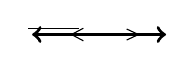
\begin{tikzpicture}\draw[<->,very thick](0,0)--(1.7,0);\draw(-.05,.08)--(.6,.08);\draw(.65,.08)--(.5,0)--(.65,-.08);\draw(1.2,.07)--(1.35,0)--(1.2,-.07);\end{tikzpicture}}
\margin{deg ext}
\diagram{\begin{tikzcd}[column sep=large,row sep=large]
 A_n^0\simeq k\{\{T\}\}\{\{X_0,\ldots,X_n\}\}/(\sum X_i-T)_{pd}\arrow[d,equal]
 &k\{\{T\}\}\{\{X_0,\ldots,X_n\}\}\arrow[l,two heads,tail,"{\text{épi}}"']\arrow[d,equal]\\
 k\{\{X_0,\ldots,X_n\}\}
 &k\{\{T,X_0,\ldots,X_n\}\}\arrow[l,two heads,tail,"{\substack{X_i\mapsfrom X_i\\\sum_{0\leq i\leq n}X_i\mapsfrom T}}"']
\end{tikzcd}}
\deleted{\figure{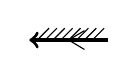
\begin{tikzpicture}\draw[<-,very thick](0,0)--(1,0);\draw(.7,.12)--(.5,0)--(.7,-.12);\foreach\x in{.1,.2,.3,.4,.5,.6,.7,.8}{\draw(\x,0)--(\x+.15,.15);}\end{tikzpicture}}}
\unsure{duals}
\diagram{\begin{tikzcd}[column sep=large,row sep=large]
 (A^n)_0\simeq k[U+Y_0,U+Y_1,\ldots,U+Y_n]\arrow[d,equal]
 &k[U][Y_0,\ldots,Y_n]\arrow[d,equal]\\
 k[Z_0,Z_1,\ldots,Z_n]\arrow[r,tail,"{Z_i\mapsto U+Y_i}"']
 &k[U,Y_0,\ldots,Y_n]
 \arrow[from=1-1,to=1-2,tail,"{\text{mono}}"]
\end{tikzcd}}
\margin{deg ext}
\margin{[l'image est \unsure{l'intersection} des noyaux des \unsure{op. diff.}
$\left(\frac{\partial}{\partial Y_0}+\cdots+\frac{\partial}{\partial Y_n}-\frac{\partial}{\partial U}\right)^{(i)}$]}
\figure{\begin{tikzpicture}\draw(0,1.5)..controls(.4,1)and(1.1,.5)..(1.6,.2);\draw(1.65,.2)--(2.3,.18);\end{tikzpicture}}
\[
\begin{aligned}
\langle X_0^{(i_0)}\cdots X_n^{(i_n)},Z_0^{j_0}\cdots Z_n^{j_n}\rangle
 &=\prod_{0\leq\alpha\leq n}\delta_{i_\alpha,j_\alpha}\\
 &=\begin{cases}0&\text{si }(i_\alpha)\ne(j_\alpha)\\1&\text{si }(i_\alpha)=(j_\alpha)\end{cases}
\end{aligned}
\]
\[
\begin{aligned}
\langle T^{(\lambda)}X_0^{(i_0)}\cdots X_n^{(i_n)},U^\mu Y_0^{j_0}\cdots Y_n^{j_n}\rangle
 &=\delta_{\lambda,\mu}\unsure{\delta_{(i_\alpha)(j_\alpha)}}\\
 &=\begin{cases}0&\text{si }(\lambda,(i_\alpha))\ne(\mu,(j_\alpha))\\1&\text{si }\text{---}=\text{---}\end{cases}
\end{aligned}
\]

\margin{degré tot = deg ext\quad i.e. \unsure{deg compl.}$=0$}
\diagram{\begin{tikzcd}[column sep=large]
 A_n^{*=*}\simeq\bigwedge_k^*[dX_0,\ldots,dX_n]/(\sum dX_i)
 &\bigwedge_k^*[dX_0,\ldots,dX_n]\arrow[l,two heads,tail,"{\text{épi}}"']
\end{tikzcd}}
\unsure{duals}
\diagram{\begin{tikzcd}[row sep=large,column sep=large]
 (A^n)_{*=*}\simeq(\bigwedge_k^*[y_0,\ldots,y_n])^{\unsure{!|'}}\arrow[r,tail]\arrow[d,equal]
 &\bigwedge_k^*[y_0,\ldots,y_n]\\
 \bigwedge_k^*\bigl(\underbrace{[y_0,\ldots,y_n]^{\unsure{!|'}}}_{\substack{\text{ss-e.v. de}\\ky_0\oplus\cdots\oplus ky_n\\\text{formé aux vect. dont la}\\\text{somme des coord.}=0}}\bigr)&
\end{tikzcd}}
\margin{l'image est le noyau de $i_X$, où $X$ est la forme sur $ky_0\oplus\cdots\oplus ky_n$ ``somme des coordonnées'' et où $i_X$ est le prod. int.}

\uline{NB} On a un isom can
\[
\bigwedge_k^{\deleted{\unsure{*}}\unsure{n-1|n}}([y_0\ldots y_n]^{\unsure{'|!}})
\simeq\bigwedge_k^n([y_0,\ldots,y_n])\simeq k
\]
déduit de la suite exacte
\diagram{\begin{tikzcd}[column sep=small]
0\arrow[r,dash]&{[y_0,\ldots,y_n]'}\arrow[r,dash]&{[y_0,\ldots,y_n]}\arrow[r,dash]&k\arrow[r,dash]&0
\end{tikzcd}}
Donc
\[
 (A^n)_n\overset{\text{iso can}}\simeq(A^n)_0\simeq k[Z_0,\ldots,Z_n]
\]
\margin{deg ext}
\figure{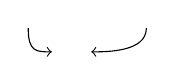
\begin{tikzpicture}\draw[->](0,.3)..controls(0,0)and(.1,0)..(.3,0);\draw[->](1.5,.3)..controls(1.5,0)and(1,0)..(.8,0);\end{tikzpicture}}
d'où
\[
\unsure{\kappa_n}:k[U]\longrightarrow k[Z_0,\ldots,Z_n]
\]
\margin{138}

\scanpage{140}
\figure{\begin{tikzpicture}[scale=.3]\draw(0,0)--(.25,-.15)--(0,-.3);\draw(-.4,-.2)--(-.5,-.25);\end{tikzpicture}}
\begin{center}- \mspage{135} -\end{center}\margin{IX}

qui montre que $\Phi$ \uline{est canoniquement isomorphe au sous-groupe de torsion de} $H^1(I,U)$.

D'autre part, de la suite exacte (11.3.3) on déduit un isomorphisme, pour tout $n=\ell^r$ :
\[
(11.3.9)\qquad H^1(I,T_n)\simeq\operatorname{Hom}(I,T_n)\xleftarrow{\sim}\operatorname{Hom}(T,T_n)\xleftarrow{\sim}\mathbb Z/n\mathbb Z
\]
(NB on fait opérer $I$ trivialement sur $T$, donc sur $T_n=T/nT$) ; d'où, pour tout $I$-$\mathbb Z_\ell$-Module fini $M$, si
\[
(11.3.10)\qquad M'=\operatorname{Hom}(M,T\otimes D_\ell)
\]
désigne son ``dual de Cartier'', un accouplement canonique
\[
(11.3.11)\qquad H^i(I,M)\otimes H^{1-i}(I,M')\longrightarrow H^1(I,T\otimes D_\ell)\simeq D_\ell,
\]
où le dernier isomorphisme est déduit des isomorphismes (11.3.9) par passage à la limite inductive sur les puissances $n$ de $\ell$. Il est bien connu que ces accouplements sont des \uline{dualités parfaites} (cf. par exemple SGA 5 I 5). Prenant dans ces accouplements $M$ de la forme $U_n$, donc $M'=U'_n$, on trouve par passage à la limite un accouplement parfait
\[
(11.3.12)\qquad H^0(I,U\otimes D_\ell)\times H^1(I,U')\longrightarrow D_\ell,
\]
où le deuxième facteur du premier membre est un $\mathbb Z_\ell$-module de type fini. Un nouveau passage à la limite dans les accouplements (11.3.12) (pour des morphismes de transition de la forme $\ell^r.\mathrm{id}$) nous donne un deuxième accouplement parfait
\[
(11.3.13)\qquad H^0(I,U\otimes\mathbb Q_\ell)\times H^1(I,U'\otimes\mathbb Q_\ell)\longrightarrow D_\ell
\]
de vectoriels de dimension finie sur $\mathbb Q_\ell$. Désignant par $i'$, $j'$ les

\margin{\figure{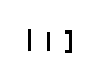
\begin{tikzpicture}[scale=.35]\draw[very thick](0,0)--(0,.8);\draw[very thick](.7,0)--(.7,.7);\draw[very thick](1.3,.7)--(1.5,.7)--(1.5,0)--(1.3,0);\end{tikzpicture}}}
\figure{\begin{tikzpicture}[scale=.3]\draw(0,0)--(0,.5);\draw(.7,0)--(.7,.35);\draw(1.5,.1)--(1.5,.65);\draw(3.4,.2)--(3.5,.5);\end{tikzpicture}}
\margin{\unsure{453}}\margin{453}\margin{139}

\scanpage{141}
$S,S^+,\gamma^*,t$
\[
 (A_n^*)^n\simeq S\unsure{\{\{}X_0,\ldots,X_n\unsure{\}\}}/(\sum X_i-t)_{pd}
 \otimes_S\underbrace{S[dX_0,\ldots,dX_n]/(\sum dX_i)}_{\substack{\text{en degré }n\\\text{c'est }\simeq S\\\text{avec la base}\\dX_0\wedge\cdots\wedge dX_{n-1}}}
\]
\diagram{\begin{tikzcd}[row sep=large]
 \unsure{\simeq}S\{X_0,\ldots,X_{n-1}\}[dX_0,\ldots,dX_{n-1}]\arrow[d,"{\unsure{\kappa^n|\pi^n}\ (S\text{-linéaire})}"]\\
 S
\end{tikzcd}}
\[
\begin{aligned}
\kappa^n(X_0^{(i_0)}\cdots X_{n-1}^{(i_{n-1})}dX_0^{\deleted{\unsure{t}}}\wedge\cdots\wedge dX_{n-1})
 &=\deleted{\unsure{\prod_\alpha i_\alpha!}}\,
 t^{\overbrace{(n+\sum i_\alpha)}^{\sum(i_\alpha+1)}}\gamma_{i_0,\ldots,i_{n-1}}
\end{aligned}
\]
où $\gamma_{i_0\ldots i_{n-1}}$ est un entier canonique
\[
\gamma_{i_0\ldots i_{n-1}}=
\frac{(n+\sum\unsure{i_\alpha})!}{\prod_\alpha(\unsure{i_\alpha!})}
\underbrace{\int\!\cdots\!\int_{\substack{\sigma_n=\{X_0,\ldots,X_{n-1}\geq0\\X_0+\cdots+X_{n-1}\leq1}}
 X_0^{i_0}\cdots X_{n-1}^{i_{n-1}}dX_0\wedge\cdots\wedge dX_{n-1}}_{\substack{0\leq\qquad\leq\frac1{n!}\gamma_{0,0,\ldots,0}\overset?=\frac1{n!}}}
\]

On peut aussi calculer par \unsure{récurrence} sur $n$, en utilisant Stokes
\[
\begin{aligned}
\kappa^n\bigl(\underbrace{X_0^{(i_0)}\cdots X_{n-1}^{(i_{n-1})}dX_0\wedge\cdots\wedge dX_{n-1}}_{d(X_{n-1}^{(i_{n-1}+1)}dX_0^{(i_0+1)}\cdots\deleted{\unsure{d}}\,dX_{n-2}^{(i_{n-2}+1)})}\bigr)
 &=\kappa^{n-1}\bigl(\partial_{ss}\underbrace{X_{n-1}^{(i_{n-1}+1)}dX_0^{(i_0+1)}\cdots}_{\substack{X_{n-1}^{(i_{n-1}+1)}dX_0^{(i_0+1)}\cdots\\d(X_{n-2}^{(i_{n-2}+1)})}}\bigr)
\end{aligned}
\]
i.e.\quad\deleted{$\unsure{\gamma}$}
\[
\deleted{\unsure{(-1)^{n-1}}}\kappa_{n-1}\Bigl(
\underbrace{\bigl(t-(X_0+\cdots+X_{n-2})\bigr)^{(i_{n-1}+1)}}_{
 \sum_{\substack{\deleted{\unsure{\lambda+\ell_0+\cdots+\ell_{n-2}}}\\\uline{\lambda}+\uline{\ell_0}+\cdots+\uline{\ell_{n-2}}=i_{n-1}+1}}
 (-1)^{\unsure{\sum\ell_\alpha}}X_0^{(\ell_0)}\cdots X_{n-2}^{\unsure{(\ell_{n-1})|(\ell_{n-2})}}t^{(\lambda)}}
 X_0^{(i_0)}\cdots X_{n-2}^{(i_{n-2})}dX_0\wedge\cdots\wedge dX_{n-2}\Bigr)
\]
\[
\begin{aligned}
&=\deleted{\unsure{(-1)^{n-1}}}\Bigl(\kappa_{n-1}\Bigl(
\sum_{\lambda+\sum_0^{n-2}\ell_\alpha=i_{n-1}+1}
 (-1)^{\sum\ell_\alpha\deleted{\unsure{+n-1}}}
 C_{i_0,\ell_0}C_{i_1,\ell_1}\cdots C_{i_{n-2},\ell_{n-2}}\\
&\hspace{3em}\inserted{\unsure{C_{\lambda,\sum_0^{n-2}(i_\alpha+\ell_\alpha+1)}}}
 t^{(\lambda)}X_0^{(i_0+\ell_0)}\cdots X_{n-2}^{(i_{n-2}+\ell_{n-2})}dX_0\wedge\cdots\wedge dX_{n-2}
\end{aligned}
\]
\[
\begin{aligned}
&=t^{\deleted{\unsure{\sum}}(n+\sum i_\alpha)}\Bigl[
 (-1)^{i_{n-1}+1}\deleted{\unsure{t}}
 \sum_{\uline{\lambda}+\sum\uline{\ell_\alpha}=i_{n-1}+1}
 (-1)^{\sum_\alpha\ell_\alpha}
 C_{i_0,\ell_0}\cdots C_{i_{n-2},\ell_{n-2}}
 \gamma_{i_0+\ell_0,\ldots,i_{n-2}+\ell_{n-2}}
\end{aligned}
\]
\figure{\begin{tikzpicture}\draw(0,.25)..controls(0,0)and(1.5,0)..(1.8,-.12)..controls(2.1,0)and(3.5,0)..(3.5,.25);\draw[->](1.8,-.15)--(1.4,-.9);\end{tikzpicture}}
Donc
\[
\begin{aligned}
\gamma_{i_0,\ldots,i_{n-1}}
 &=\deleted{(-1)^{i_{n-1}+1}}
 \sum_{\uline{\lambda}+\sum_0^{n-2}\uline{\ell_\alpha}=i_{n-1}+1}
 (-1)^{\sum_0^{n-2}\ell_\alpha}
 C_{i_0,\ell_0}\cdots C_{i_{n-2},\ell_{n-2}}\\
&\qquad\inserted{\unsure{C_{\lambda,n-1+\sum_0^{n-2}(\ell_\alpha+i_\alpha)}}}
 \gamma_{i_0+\ell_0,i_1+\ell_1,\ldots,i_{n-2}+\ell_{n-2}}
\end{aligned}
\]
\figure{\begin{tikzpicture}\draw(0,1)..controls(.2,.7)and(1,.9)..(1.3,.4);\draw(1.3,.4)..controls(1.5,.1)and(2,.2)..(2.3,0);\end{tikzpicture}}
\margin{140}
